\documentclass[a4paper,spanish,11pt]{article}
\usepackage{booktabs}% http://ctan.org/pkg/booktabs
\usepackage{mathpazo}
\usepackage[utf8]{inputenc} % Required for inputting international characters
\usepackage[T1]{fontenc} % Output font encoding for international characters%
%\usepackage{xcolor,colortbl} %Para colorear las columnas de las tablas.
\usepackage{tabularx}
\usepackage{float}
\usepackage{graphicx}
\usepackage{csquotes}
\usepackage{multirow}	%Para combinar varias filas en una tabla.
%\definecolor{Gray}{gray}{0.9}
%\newcolumntype{a}{>{\columncolor{Gray}}c}

\usepackage{array}

\newcolumntype{L}[1]{>{\raggedright\let\newline\\\arraybackslash\hspace{0pt}}m{#1}}
\newcolumntype{C}[1]{>{\centering\let\newline\\\arraybackslash\hspace{0pt}}m{#1}}
\newcolumntype{R}[1]{>{\raggedleft\let\newline\\\arraybackslash\hspace{0pt}}m{#1}}


%Para poder usar bullet adentro de una tabla 
\newcommand{\tabitem}{~~\llap{\textbullet}~~}


%opening
\title{Guía del nuevo conjunto de comandos}
\author{Felipe Costa}

\begin{document}

\maketitle

\renewcommand{\contentsname}{Contenido}
\tableofcontents

\newpage

%\section{Guía del nuevo conjunto de comandos}

En este apéndice se presentan, en primer lugar, las conexiones \textit{hardware} necesarias para poder establecer la comunicación con el ESP8266-01, utilizando la placa de alimentación. Luego, se presenta la sintaxis de los comandos y la definición de cada uno de ellos. El objetivo de este apéndice es actuar como una guía para las personas que quieren empezar a utilizar el ESP8266-01 con el nuevo conjunto de comandos.

\section{Conexiones hardware}
Para comunicar el microcontrolador externo y el módulo ESP8266-01, se utiliza el periférico UART, con una velocidad por defecto de 115200 bps. Además, si se utiliza la placa de alimentación desarrollada, en necesario disponer de un puerto GPIO en el microcontrolador, para controlar la activación del regulador en la placa de alimentación. El diagrama de conexión se muestra en la figura \ref{fig:conexion_mcu_placa_alimentacion}. 

\begin{figure}[H]
	\centering
	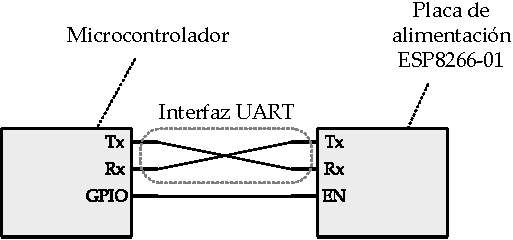
\includegraphics[scale=1]{conexion_mcu_placa_alimentacion.pdf}
	\caption{Diagrama de conexión entre el microcontrolador externo y la placa de alimentación para el ESP8266-01.}
	\label{fig:conexion_mcu_placa_alimentacion}
\end{figure}

Por motivos de simplicidad, no se muestran las conexiones de la fuente, que también son necesarios para suministrar energía al microcontrolador y la placa de alimentación. La placa de alimentación para el ESP8266-01 debe ser alimentado con un voltaje mínimo de 3,6 V y 6 V como máximo. En cuanto a la corriente, si bien el consumo de corriente promedio es de 80 mA, la fuente debe ser capaz de entregar hasta 500mA, según recomendaciones del fabricante \cite{ESP8266SYSDESCRIPTION}.

\section{Esquema de comunicación}
El esquema de comunicación es del tipo comando-respuesta. El microcontrolador envía un comando al módulo ESP8266-01, este procesa y realiza las acciones correspondientes al comando recibido, genera una respuesta y la envía al microcontrolador. No se admiten mensajes no solicitados en este esquema, es decir, el módulo ESP8266-01 no puede enviar un mensaje al microcontrolador si este no envía primero un comando, siendo la única excepción, cuando el módulo ESP8266-01 es reiniciado de forma inesperada, en ese caso, el módulo envía una cantidad de caracteres, finalizando con los caracteres %\enquote{{\ttfamily R\textbackslash n}}.

\section{Resumen de comandos}
En las tablas \ref{tab:comandos_basicos}, \ref{tab:comandos_wifi} y \ref{tab:coomnados_tcpip} se presentan todos los comandos disponibles y una breve descripción de la función de cada uno.


\begin{table}[H]
	\centering
	\renewcommand\arraystretch{1.5}
	\begin{tabular}{@{} ll @{}}
		\toprule
		\textbf{Comando} & \textbf{Descripción} \\ 
		\midrule
		MIS & Verifica el funcionamiento del módulo. \\
		MRS & Reinicia el módulo. \\
		MVI & Retorna la versión actual del \textit{firmware}. \\
		MDS & Configura el modo de bajo consumo \textit{deep-sleep}. \\
		MUC & Configura la velocidad de transmisión UART. \\
		MRP & Configura la potencia de transmisión RF. \\ 
		MFH & Retorna cantidad de bytes disponibles en la memoria RAM. \\
		\bottomrule
	\end{tabular}
	\caption{Comandos Básicos.}
	\label{tab:comandos_basicos}
\end{table}


\begin{table}[H]
	\centering
	\renewcommand\arraystretch{1.5}
	\begin{tabular}{@{} ll @{}}
		\toprule
		\textbf{Comando} & \textbf{Descripción} \\ 
		\midrule
		WFM & Establece el modo WiFi del módulo.\\
		WFC & Conecta a un AP en modo estación.\\ 
		WFS & Retorna el SSID de los puntos de acceso en rango. \\ 
		WFD & Desconecta al módulo del AP.\\
		WFA & Configura el módulo como un AP.\\
		WSI & Retorna información acerca de la interfaz AP. \\
		WAD & Desactiva el AP del módulo. \\ 
		WCF & Desactiva DHCP en modo estación, configuración estática. \\
		WAC & Configura los parámetros de red del AP. \\
		WMA & Configura la dirección MAC del módulo.\\
		WSC & Inicia SmartConfig. \\
		WSS & Detiene SmartConfig. \\ 
		WSD & Retorna estado SmartConfig. \\ 
		WSN & Configura el \textit{hostname} del módulo. \\
		WRI & Retorna el RSSI. \\
		WID & Retorna el SSID del AP al cual se encuentra conectado. \\ 
		\bottomrule
	\end{tabular}
	\caption{Comandos WiFi.}
	\label{tab:comandos_wifi}
\end{table}

\begin{table}[H]
	\centering
	\renewcommand\arraystretch{1.5}
	\begin{tabular}{@{} ll @{}}
		\toprule
		\textbf{Comando} & \textbf{Descripción} \\ 
		\midrule
		SOI & Retorna información acerca de una conexión. \\
		IDN & Retorna la dirección IP a partir de un nombre de dominio. \\
		CCS & Inicia una conexión, en modo cliente.  \\
		SOW & Envía datos a través de una conexión TCP. \\
		SOR & Recibe datos a través de una conexión TCP. \\
		SOC & Cierra una conexión TCP. \\ 
		WFI & Retorna la configuración de red actual del modo estación. \\
		WAI & Retorna la configuración de red actual del modo AP. \\
		SLC & Crea un servidor TCP en el módulo. \\
		SAC & Acepta clientes que desean conectarse a un servidor. \\ 
		SCC & Detiene un servidor TCP. \\ 
		SVU & Crea un servidor UDP. \\ 
		SDU & Envía datos utilizando el protocolo UDP. \\
		RVU & Recibe datos utilizando el protocolo UDP. \\ 
		STC & Configura el servidor SNTP. \\ 
		STG & Obtiene el tiempo actual del servidor SNTP. \\
		\bottomrule
	\end{tabular}
	\caption{Comandos TCP/IP.}
	\label{tab:coomnados_tcpip}
\end{table}

\section{Sintaxis de los comandos}

\paragraph{Comandos.} En cuanto a los comandos que puede recibir el ESP8266-01, la sintaxis es la siguiente: \\ 

\begin{tt}
	<comando>,<parámetro1>,<parámetro2>, . . ,<parámetroN> \textbackslash n
\end{tt}
\\

En donde: 
\begin{itemize}
	\item Los caracteres permitidos serán aquellos del conjunto de caracteres ASCII, con la excepción de los comandos para enviar y recibir datos TCP/UDP.
	\item 
	\begin{ttfamily}
		<comando>
	\end{ttfamily} es el nombre del comando. Debe estar en letras mayúsculas y poseer una longitud de tres caracteres.
	\item \begin{ttfamily}
		<parámetro1>,<parámetro2>, . . ,<parámetroN> 
	\end{ttfamily} son los parámetros del comando. Cada comando especifica la cantidad de parámetros que necesita. Pueden existir comandos que no necesitan de ningún parámetro.
	\item Los comandos que requieren parámetros, deben utilizar el carácter \enquote*{{\ttfamily ,}} para separar cada parámetro.
	\item El carácter de nueva línea ({\ttfamily \textbackslash n}) se utiliza para indicar el final de un comando.  
\end{itemize}

\paragraph{Respuestas.}En cuanto a las respuestas a los comandos, existen 4 tipos de respuestas: 
\begin{enumerate}
	\item	Comando ejecutado con éxito:\\
	{\ttfamily 0\textbackslash n}
	\item	Comando que produjo un error, retorna un solo carácter numérico positivo, mayor que 0 y menor que 10:\\
	{\ttfamily <numero\_error>\textbackslash n} 
	\item	Comando ejecutado con éxito y que retorna información:\\	\begin{ttfamily} 0,<información1>,<información2>, . . ,<informaciónN> \textbackslash n \end{ttfamily}
	\item   Comando ejecutado con éxito que retorna información y datos:\\ \begin{ttfamily} 0,<información>,<datos>\textbackslash n \end{ttfamily}
\end{enumerate}
Al igual que los comandos, se utiliza el carácter de nueva linea ({\ttfamily \textbackslash n}) para indicar el final de una respuesta. Además, los campos son separados con el carácter \enquote*{{\ttfamily ,}}.

\paragraph{Consideraciones.}

Los caracteres \begin{ttfamily}<>\end{ttfamily} no forman parte del conjunto, se utilizan únicamente de manera representativa. 

El carácter de nueva línea ({\ttfamily \textbackslash n}) se asume que ocupa un solo Byte\footnote{Unidad de información de base utilizada en computación, equivalente a un conjunto ordenado de 8 bits} y se traduce a un solo valor tipo {\ttfamily char}, según el estándar del lenguaje C.

\section{Definición de los comandos}

\subsection{Comandos Básicos}

\begin{table}[H]
	\centering
	\begin{tabular}{@{} L{2.2cm}L{3.2cm}L{7cm} @{}}
		\toprule
		\multicolumn{3}{c}{\textbf{Comando MIS}}\\
		\midrule
		\multirow{5}{=}{\textbf{Descripción}} & \multicolumn{2}{ p{10.5cm} }{Comando utilizado para verificar que el módulo se encuentra funcionando correctamente y está listo para recibir comandos. En caso de no recibir respuesta al ejecutar este comando, dentro de un periodo de 20 milisegundos, significa que el módulo no responde y es necesario reiniciarlo.} \\ 
		\midrule
		\textbf{Sintaxis} & \multicolumn{2}{l}{{\ttfamily MIS\textbackslash n}}\\
		\midrule
		\textbf{Parámetros} & \multicolumn{2}{l}{Ninguno.} \\
		\midrule 
		\textbf{Respuesta} & \tabitem \ttfamily 0\textbackslash n & El módulo está activo y listo para recibir comandos.\\
		\bottomrule
	\end{tabular}
	\caption{Definición del comando MIS.}
\end{table}




%\subsubsection*{MIS}
%Comando utilizado para verificar que el módulo se encuentra funcionando correctamente y está listo para recibir comandos. En caso de no recibir respuesta al ejecutar este comando, dentro de un periodo de 20 milisegundos, significa que el módulo no responde y es necesario reiniciarlo.
%\begin{itemize}
%	\item \textbf{Sintaxis}\\
%	{\ttfamily MIS\textbackslash n}
%	\item \textbf{Parámetros}\\
%	Ninguno.
%	\item \textbf{Respuesta}\\
%	{\ttfamily 0\textbackslash n}
%\end{itemize}

\begin{table}[H]
	\centering
	\begin{tabular}{@{} L{2.2cm}L{3.2cm}L{7cm} @{}}
		\toprule
		\multicolumn{3}{c}{\textbf{Comando MRS}}\\
		\midrule
		\multirow{4}{=}{\textbf{Descripción}} & \multicolumn{2}{ p{10.5cm} }{Comando que reinicia inmediatamente el módulo. Al iniciar de vuelta el módulo, este envía por el puerto serial una serie de caracteres, luego de esto se recibe el carácter {\ttfamily R\textbackslash n}, el cual indica que el módulo está listo.} \\ 
		\midrule
		\textbf{Sintaxis} & \multicolumn{2}{l}{{\ttfamily MRS\textbackslash n}}\\
		\midrule
		\textbf{Parámetros} & \multicolumn{2}{l}{Ninguno.} \\
		\midrule 
		\textbf{Respuesta} & \tabitem \ttfamily R\textbackslash n & El módulo fue reiniciado correctamente y está listo para recibir comandos.\\
		\bottomrule
	\end{tabular}
	\caption{Definición del comando MRS.}
\end{table}

%\subsubsection*{MRS}
%Comando que reinicia inmediatamente el módulo. Al iniciar de vuelta el módulo, este envía por el puerto serial una serie de caracteres, luego de esto se recibe el carácter {\ttfamily R\textbackslash n}, el cual indica que el módulo está listo.
%\begin{itemize}
%	\item \textbf{Sintaxis}\\
%	{\ttfamily MRS\textbackslash n}
%	\item \textbf{Parámetros}\\
%	Ninguno.
%	\item \textbf{Respuesta}\\
%	{\ttfamily R\textbackslash n}
%\end{itemize}

\begin{table}[H]
	\centering
	\begin{tabular}{@{} L{2.2cm}L{3.2cm}L{7cm} @{}}
		\toprule
		\multicolumn{3}{c}{\textbf{Comando MVI}}\\
		\midrule
		\multirow{4}{=}{\textbf{Descripción}} & \multicolumn{2}{ p{10.5cm} }{Comando que retorna información acerca de la versión actual del \textit{firmware} que se está ejecutando en el módulo. También informa acerca de la versión del Arduino Core utilizado para crear el \textit{firmware}.} \\ 
		\midrule
		\textbf{Sintaxis} & \multicolumn{2}{l}{{\ttfamily MVI\textbackslash n}}\\
		\midrule
		\textbf{Parámetros} & \multicolumn{2}{l}{Ninguno.} \\
		\midrule 
		\textbf{Respuesta} &  \multicolumn{2}{l}{\tabitem \ttfamily 0,Firmware:<numero\_version>,ArduinoCore:<version>\textbackslash n}\\
		\bottomrule
	\end{tabular}
	\caption{Definición del comando MVI.}
\end{table}


%\subsubsection*{MVI}
%Comando que retorna información acerca de la versión actual del \textit{firmware} que se está ejecutando en el módulo. También informa acerca de la versión del Arduino Core utilizado para crear el \textit{firmware}.
%\begin{itemize}
%	\item \textbf{Sintaxis}\\
%	{\ttfamily MVI\textbackslash n}
%	\item \textbf{Parámetros}\\
%	Ninguno.
%	\item \textbf{Respuesta}\\
%	{\ttfamily 0,F:<numero\_version>,A:<version>\textbackslash n}
%\end{itemize}

\begin{table}[H]
	\centering
	\begin{tabular}{@{} L{2.2cm}L{3.2cm}L{7cm} @{}}
		\toprule
		\multicolumn{3}{c}{\textbf{Comando MDS}}\\
		\midrule
		\multirow{2}{=}{\textbf{Descripción}} & \multicolumn{2}{ p{10.5cm} }{Comando que configura el modo de bajo consumo \textit{Deep-sleep} para el módulo.} \\ 
		\midrule
		\textbf{Sintaxis} & \multicolumn{2}{l}{ {\ttfamily MDS,tiempo\_dormir,modo\_rf\textbackslash n} }\\
		\midrule
		\multirow{11}{=}{\textbf{Parámetros}} & \tabitem \ttfamily tiempo\_dormir & El tiempo medido en $us$ que el dispositivo estará en deep-sleep.\\
		\cmidrule(lr){2-3}
		& \multirow{9}{=}{\tabitem \ttfamily modo\_rf}  & \tabitem \textbf{0}: Configuración RF por defecto.\\
		& & \tabitem \textbf{1}: Efectuar calibración RF.\\
		& & \tabitem \textbf{2}: No se realiza calibración RF, esto reduce el consumo de corriente.\\
		& & \tabitem \textbf{3}: Desactiva el sistema de RF al despertarse. Esta opción permite el menor consumo posible de corriente, sin embargo, no se pueden enviar ni recibir datos al despertarse.\\		
		\midrule 
		\multirow{2}{=}{\textbf{\textbf{Respuesta}}} & \tabitem \ttfamily 0\textbackslash n & Configuración exitosa.\\
		\cmidrule(lr){2-3}
		& \tabitem \ttfamily 1\textbackslash n & Configuración no aplicada.\\
		\bottomrule
	\end{tabular}
	\caption{Definición del comando MDS.}
\end{table}


%\subsubsection*{MDS}
%Comando que configura el modo de bajo consumo \textit{Deep-sleep} para el módulo.
%\begin{itemize}
%	\item \textbf{Sintaxis}\\
%	{\ttfamily MDS,\textless tiempo\_dormir\textgreater,\textless modo\_rf\textgreater\textbackslash n}
%	\item \textbf{Parámetros}
%	\begin{itemize}
%		\item{\ttfamily \textless tiempo\_dormir\textgreater}\\
%		El tiempo medido en $us$ que el dispositivo estara en deep-sleep.
%		\item{\ttfamily \textless modo\_rf\textgreater}\\
%		Parámetro que determina el comportamiento de la calibración RF luego de despertarse.
%		\begin{itemize}
%			\item \textbf{0} , Configuración RF por defecto. 
%			\item \textbf{1} , Efectuar calibración RF.
%			\item \textbf{2} , No se realiza calibración RF, esto reduce el consumo de corriente.
%			\item \textbf{3} , Desactiva el sistema de RF al despertarse. Esta opción permite el menor consumo posible de corriente, sin embargo, no se pueden enviar ni recibir datos al despertarse.
%		\end{itemize}
%	\end{itemize}
%\end{itemize}

\begin{table}[H]
	\centering
	\begin{tabular}{@{} L{2.2cm}L{3.2cm}L{7cm} @{}}
		\toprule
		\multicolumn{3}{c}{\textbf{Comando MUC}}\\
		\midrule
		\multirow{3}{=}{\textbf{Descripción}} & \multicolumn{2}{ p{10.5cm} }{Comando utilizado para modificar la velocidad de transmisión del periférico UART, utilizado por el módulo para comunicarse con el microcontrolador externo.} \\ 
		\midrule
		\textbf{Sintaxis} & \multicolumn{2}{l}{{\ttfamily MUC,velocidad\textbackslash n}}\\
		\midrule
		\multirow{1}{=}{\textbf{Parámetros}} & \ttfamily velocidad &  Velocidad de transmisión deseada. El rango permitido para este parámetro va desde 9600 a 921600.\\
		\midrule 
		\multirow{3}{=}{\textbf{Respuesta}} & \tabitem \ttfamily 0\textbackslash n & El cambio de velocidad se realizó con éxito. Es necesario esperar 5 ms para enviar el siguiente comando utilizando la nueva velocidad.\\
		\cmidrule(lr){2-3}
		& \tabitem \ttfamily 1\textbackslash n & Error, el parámetro {\ttfamily \textless velocidad\textgreater} se encuentra fuera de rango. \\
		\bottomrule
	\end{tabular}
	\caption{Definición del comando MUC.}
\end{table}

%\subsubsection*{MUC}
%Comando utilizado para modificar la velocidad de transmisión del periférico UART, utilizado por el módulo para comunicarse con el microcontrolador externo.
%\begin{itemize}
%	\item \textbf{Sintaxis}\\
%	{\ttfamily MUC,\textless velocidad\textgreater\textbackslash n}
%	\item \textbf{Parámetros}
%	\begin{itemize}
%		\item{\ttfamily \textless velocidad\textgreater}\\
%		Velocidad de transmisión deseada. El rango permitido para este parámetro va desde 9600 a 921600. 
%	\end{itemize}
%	\item \textbf{Respuesta}
%	\begin{itemize}
%		\item {\ttfamily 0\textbackslash n} \\
%		El cambio de velocidad se realizó con éxito. Es necesario esperar 5 ms para enviar el siguiente comando utilizando la nueva velocidad.
%		\item{\ttfamily 1\textbackslash n} \\
%		Error, el parámetro {\ttfamily \textless velocidad\textgreater}  se encuentra fuera de rango. 
%	\end{itemize}
%\end{itemize}

\begin{table}[H]
	\centering
	\begin{tabular}{@{} L{2.2cm}L{3.2cm}L{7cm} @{}}
		\toprule
		\multicolumn{3}{c}{\textbf{Comando MRP}}\\
		\midrule
		\multirow{2}{=}{\textbf{Descripción}} & \multicolumn{2}{ p{10.5cm} }{Comando que configura la potencia de transmisión de la antena de radio frecuencia (RF) del módulo.} \\ 
		\midrule
		\textbf{Sintaxis} & \multicolumn{2}{l}{{\ttfamily MRP,potencia\_dbm\textbackslash n}}\\
		\midrule
		\multirow{1}{=}{\textbf{Parámetros}} & \ttfamily potencia\_dbm & Potencia de transmisión a ser utilizada, en $dBm$. El rango de valores permitido va desde 0 a 20,5.\\
		\midrule 
		\multirow{3}{=}{\textbf{Respuesta}} & \tabitem \ttfamily 0\textbackslash n & La configuración fue aplicada con éxito.\\
		\cmidrule(lr){2-3}
		& \tabitem \ttfamily 1\textbackslash n & El parámetro {\ttfamily potencia\_dbm} está fuera de rango. \\
		\bottomrule
	\end{tabular}
	\caption{Definición del comando MRP.}
\end{table}

%\subsubsection*{MRP}
%Comando que configura la potencia de transmisión de la antena de radio frecuencia (RF) del módulo.
%\begin{itemize}
%	\item \textbf{Sintaxis}\\
%	{\ttfamily MRP,potencia\_dbm\textbackslash n}
%	\item \textbf{Parámetros}\\
%	\begin{itemize}
%		\item{\ttfamily potencia\_dbm}\\
%		Potencia de transmisión a ser utilizada, en $dBm$. El rango de valores permitido va desde 0 a 20,5. 
%	\end{itemize}
%	\item \textbf{Respuesta}
%	\begin{itemize}
%		\item {\ttfamily 0\textbackslash n} \\
%		La configuración fue aplicada con éxito.
%		\item {\ttfamily 1\textbackslash n} \\
%		El parámetro {\ttfamily potencia\_dbm} esta fuera de rango.
%	\end{itemize}
%\end{itemize}

\begin{table}[H]
	\centering
	\begin{tabular}{@{} L{2.2cm}L{3.2cm}L{7cm} @{}}
		\toprule
		\multicolumn{3}{c}{\textbf{Comando MFH}}\\
		\midrule
		\multirow{2}{=}{\textbf{Descripción}} & \multicolumn{2}{ p{10.5cm} }{Comando que retorna la cantidad de Bytes disponibles en la memoria RAM.} \\ 
		\midrule
		\textbf{Sintaxis} & \multicolumn{2}{l}{ {\ttfamily MFH\textbackslash n} }\\
		\midrule
		\textbf{Parámetros} & \multicolumn{2}{l}{Ninguno.} \\
		\midrule 
		\textbf{Respuesta} &  \multicolumn{2}{l}{\tabitem \ttfamily 0,cantidad\_bytes\_disponibles\textbackslash n}\\
		\bottomrule
	\end{tabular}
	\caption{Definición del comando MFH.}
\end{table}

%\subsubsection*{MFH}
%Comando que retorna la cantidad de Bytes disponibles en la memoria RAM.
%\begin{itemize}
%	\item \textbf{Sintaxis}\\
%	{\ttfamily MFH\textbackslash n}
%	\item \textbf{Parámetros}\\
%	Ninguno.
%	\item \textbf{Respuesta}\\
%	{\ttfamily 0,cantidad\_bytes\_disponibles\textbackslash n}
%\end{itemize}


\subsection{Comandos WiFi}

%\begin{table}[H]
%	\centering
%	\begin{tabular}{@{} ll @{}}
%		\toprule
%		\multicolumn{2}{c}{Descripción}\\
%		\midrule
%		Comando utilizado para establecer el modo de funcionamiento WiFi del modulo.
%		mboo & mbo \\ 
%		\tabitem mbo \tabitem jf & hmmya \\ 
%		\bottomrule
%	\end{tabular}
%\end{table}


\begin{table}[H]
	\centering
	\begin{tabular}{@{} L{2.2cm}L{3.2cm}L{7cm} @{}}
		\toprule
		\multicolumn{3}{c}{\textbf{Comando WFM}}\\
		\midrule
		\multirow{2}{=}{\textbf{Descripción}} & \multicolumn{2}{ p{9cm} }{Comando utilizado para establecer el modo de funcionamiento WiFi del módulo.} \\ 
		\midrule
		\textbf{Sintaxis} & \multicolumn{2}{l}{{\ttfamily WFM,modo\_wifi\textbackslash n}}\\
		\midrule
		\multirow{5}{=}{\textbf{Parámetros}} & \multirow{5}{*}{{\ttfamily modo\_wifi}} &  \tabitem \textbf{0}: WiFi apagado. \\
		& & \tabitem \textbf{1}: Modo estación (STA). \\
		& & \tabitem \textbf{2}: Modo punto de acceso (AP). \\
		& & \tabitem \textbf{3}: Modo estación + punto de acceso (STA + AP). \\ 
		\midrule
		\multirow{5}{=}{\textbf{Respuesta}} & \tabitem \ttfamily 0\textbackslash n & La configuración fue aplicada con éxito.\\
		\cmidrule(lr){2-3}
		& \tabitem \ttfamily 1\textbackslash n & Error, el parámetro {\ttfamily modo\_wifi} se encuentra fuera de rango. \\
		\cmidrule(lr){2-3}
		& \tabitem \ttfamily 2\textbackslash n & Error, no se pudo aplicar la configuración. \\
		\bottomrule
	\end{tabular}
	\caption{Definición del comando WFM.}
\end{table}


%\subsection{WFM}
%Comando utilizado para establecer el modo de funcionamiento WiFi del módulo. 
%\begin{itemize}
%	\item \textbf{Sintaxis}\\
%	{\ttfamily WFM,modo\_wifi\textbackslash n}
%	\item \textbf{Parámetros}
%	\begin{itemize}
%		\item{\ttfamily modo\_wifi}\\
%		Parámetro que determina cual modo sera utilizado. Valores permitidos del 0 al 3. 
%		\begin{itemize}
%			\item \textbf{0} , WiFi apagado. 
%			\item \textbf{1} , modo estación (STA).
%			\item \textbf{2} , modo punto de acceso (AP).
%			\item \textbf{3} , modo estación + punto de acceso (STA + AP).
%		\end{itemize}
%	\end{itemize}
%	\item \textbf{Respuesta}
%	\begin{itemize}
%		\item{\ttfamily 0\textbackslash n} \\
%		Configuración exitosa.
%		\item{\ttfamily 1\textbackslash n} \\
%		Error, el parámetro {\ttfamily modo\_wifi} se encuentra fuera de rango.
%		\item{\ttfamily 2\textbackslash n} \\
%		Error, no se pudo establecer la configuración.
%	\end{itemize}
%\end{itemize}

\begin{table}[H]
	\centering
	\begin{tabular}{@{} L{2.2cm}L{3.2cm}L{7cm} @{}}
		\toprule
		\multicolumn{3}{c}{\textbf{Comando WFC}}\\
		\midrule
		\multirow{2}{=}{\textbf{Descripción}} & \multicolumn{2}{ p{10.5cm} }{Comando utilizado para conectar el módulo a un punto de acceso (AP, por sus siglas en inglés)} \\ 
		\midrule
		\textbf{Sintaxis} & \multicolumn{2}{l}{ {\ttfamily WFC,ssid,contraseña\textbackslash n} }\\
		\midrule
		\multirow{4}{=}{\textbf{Parámetros}} & \tabitem \ttfamily ssid & Nombre del punto de acceso al cual se desea conectar el módulo.\\
		\cmidrule(lr){2-3}
		& \tabitem \ttfamily contraseña & Contraseña del punto de acceso al cual se desea conectar el módulo.\\		
		\midrule 
		\multirow{8}{=}{\textbf{\textbf{Respuesta}}} & \tabitem \ttfamily 0\textbackslash n & Conexión exitosa.\\
		\cmidrule(lr){2-3}
		& \tabitem \ttfamily 1\textbackslash n & Error, no se pudo establecer la conexión al punto de acceso.\\
		\cmidrule(lr){2-3}
		& \tabitem \ttfamily 2\textbackslash n & Error, se alcanzó el tiempo de espera máximo (20 segundos) sin poder establecer la conexión.\\
		\cmidrule(lr){2-3}
		& \tabitem \ttfamily 3\textbackslash n & Error, contraseña incorrecta.\\
		\cmidrule(lr){2-3}
		& \tabitem \ttfamily 4\textbackslash n & Error, no se encuentra el punto de acceso.\\
		\bottomrule
	\end{tabular}
	\caption{Definición del comando WFC.}
\end{table}

%\subsection{WFC}
%Comando utilizado para conectar el módulo a un punto de acceso (AP, por sus siglas en ingles). 
%\begin{itemize}
%	\item \textbf{Sintaxis}\\
%	{\ttfamily WFC,\textless ssid\textgreater,\textless contraseña\textgreater\textbackslash n}
%	\item \textbf{Parámetros}
%	\begin{itemize}
%		\item{\ttfamily \textless ssid\textgreater}\\
%		Nombre del punto de acceso al cual se desea conectar el módulo.
%		\item{\ttfamily \textless contraseña\textgreater}\\
%		Contraseña del punto de acceso al cual se desea conectar el módulo.
%	\end{itemize}
%	\item \textbf{Respuesta}
%	\begin{itemize}
%		\item{\ttfamily 0\textbackslash n} \\
%		Conexión exitosa.
%		\item{\ttfamily 1\textbackslash n} \\
%		Error, no se pudo establecer la conexión al punto de acceso.
%		\item{\ttfamily 2\textbackslash n} \\
%		Error, se alcanzo el tiempo de espera máximo (20 segundos) sin poder establecer la conexión.
%		\item{\ttfamily 3\textbackslash n} \\
%		Error, contraseña incorrecta.
%		\item{\ttfamily 4\textbackslash n} \\
%		Error, no se encuentra el punto de acceso. 
%	\end{itemize}
%\end{itemize}

\begin{table}[H]
	\centering
	\begin{tabular}{@{} L{2.2cm}L{3.2cm}L{7cm} @{}}
		\toprule
		\multicolumn{3}{c}{\textbf{Comando WFS}}\\
		\midrule
		\multirow{2}{=}{\textbf{Descripción}} & \multicolumn{2}{ p{10.5cm} }{Comando utilizado para escanear los puntos de acceso que se encuentran al alcance del módulo.} \\ 
		\midrule
		\textbf{Sintaxis} & \multicolumn{2}{l}{ {\ttfamily WFS\textbackslash n} }\\
		\midrule
		\textbf{Parámetros} & \multicolumn{2}{l}{Ninguno.} \\	
		\midrule 
		\multirow{3}{=}{\textbf{\textbf{Respuesta}}} & \multicolumn{2}{l}{\tabitem \ttfamily 0,ssid\_1;rssi\_1,ssid\_2;rssi\_2,ssid\_N;rssi\_N\textbackslash n}\\
		& \multicolumn{2}{ p{10.5cm} }{Se retorna una lista con el SSID y RSSI de cada AP encontrado.} \\
		\cmidrule(lr){2-3}
		& \tabitem \ttfamily 1\textbackslash n & No se encontró ningún AP.\\
		\bottomrule
	\end{tabular}
	\caption{Definición del comando WFS.}
\end{table}


%\subsection{WFS}
%Comando utilizado para escanear los puntos de acceso que se encuentran al alcance del modulo.
%\begin{itemize}
%	\item \textbf{Sintaxis}\\
%	{\ttfamily WFS\textbackslash n}
%	\item \textbf{Parámetros}\\
%	Ninguno.
%	\item \textbf{Respuesta}\\
%	{\ttfamily 0,ssid\_1;rssi\_1,ssid\_2;rssi\_2,ssid\_N;rssi\_N\textbackslash n}
%	\item \textbf{Respuesta}\\
%	{\ttfamily 1\textbackslash n}\\
%	No se encontró ningún punto de acceso.
%	\item\textbf{Ejemplo}\\
%	Comando: {\ttfamily WFS\textbackslash n}\\
%	Respuesta: {\ttfamily 0,DEI-UCA;-81,DICIA-UCA;-70,LED-UCA;-85\textbackslash n}
%\end{itemize}

\begin{table}[H]
	\centering
	\begin{tabular}{@{} L{2.2cm}L{3.2cm}L{7cm} @{}}
		\toprule
		\multicolumn{3}{c}{\textbf{Comando WFD}}\\
		\midrule
		\multirow{2}{=}{\textbf{Descripción}} & \multicolumn{2}{ p{10.5cm} }{Comando utilizado para desconectar el módulo del punto de acceso al cual se encuentra conectado actualmente.}\\ 
		\midrule
		\textbf{Sintaxis} & \multicolumn{2}{l}{ {\ttfamily WFD,wifi\_off\textbackslash n} }\\
		\midrule
		\multirow{2}{=}{\textbf{Parámetros}} & \multirow{2}{*}{{\ttfamily modo\_wifi}} & Parámetro que determina si se apaga o no la radio WiFi, luego de desconectarse. \newline  \tabitem \textbf{0}: La radio WiFi sigue activada.\\
		& & \tabitem \textbf{1}: Se desactiva la radio WiFi. \\
		\midrule 
		\multirow{5}{=}{\textbf{\textbf{Respuesta}}} & \tabitem \ttfamily 0\textbackslash n & Configuración exitosa.\\
		\cmidrule(lr){2-3}
		& \tabitem \ttfamily 1\textbackslash n & Error, el parámetro {\ttfamily  wifi\_off} se encuentra fuera de rango.\\
		\cmidrule(lr){2-3}
		& \tabitem \ttfamily 2\textbackslash n & Error, no se pudo aplicar la configuración.\\
		\bottomrule
	\end{tabular}
	\caption{Definición del comando WFD.}
\end{table}

%\subsection{WFD}
%Comando utilizado para desconectar el modulo del punto de acceso al cual se encuentra conectado actualmente. 
%\begin{itemize}
%	\item \textbf{Sintaxis}\\
%	{\ttfamily WFD,wifi\_off\textbackslash n}
%	\item \textbf{Parámetros}
%	\begin{itemize}
%		\item{\ttfamily wifi\_off}\\
%		Parámetro que determina si se apagara la radio WiFi luego de desconectarse. Valores permitidos: 0 o 1.
%		\begin{itemize}
%			\item \textbf{0} , la radio WiFi sigue activada. 
%			\item \textbf{1} , se desactiva la radio WiFi.
%		\end{itemize}
%	\end{itemize}
%	\item \textbf{Respuesta}
%	\begin{itemize}
%		\item{\ttfamily 0\textbackslash n} \\
%		Configuración exitosa.
%		\item{\ttfamily 1\textbackslash n} \\
%		Error, el parámetro {\ttfamily  wifi\_off} se encuentra fuera de rango.
%		\item{\ttfamily 2\textbackslash n} \\
%		Error, no se pudo aplicar la configuración.
%	\end{itemize}
%\end{itemize}

\begin{table}[H]
	\centering
	\begin{tabular}{@{} L{2.2cm}L{3.2cm}L{7cm} @{}}
		\toprule
		\multicolumn{3}{c}{\textbf{Comando WFA}}\\
		\midrule
		\multirow{2}{=}{\textbf{Descripción}} & \multicolumn{2}{ p{10.5cm} }{Comando utilizado para configurar el módulo como un punto de acceso. El modo de autenticación es WPA2-PSK.} \\ 
		\midrule
		\textbf{Sintaxis} & \multicolumn{2}{l}{ {\ttfamily WFA,ssid,contraseña,canal,ssid\_oculto,max\_con\textbackslash n} }\\
		\midrule
		\multirow{14}{=}{\textbf{Parámetros}} & \tabitem \ttfamily ssid & Nombre del punto de acceso, longitud máxima de 63 caracteres.\\
		\cmidrule(lr){2-3}
		& \tabitem \ttfamily contraseña & Contraseña del punto de acceso, longitud mínima de 8 caracteres. \\	
		\cmidrule(lr){2-3}
		& \tabitem \ttfamily canal & Número del canal WiFi que utilizará el punto de acceso. Valores permitidos del 1 al 13.\\	
		\cmidrule(lr){2-3}
		& \tabitem \ttfamily ssid\_oculto & Parámetro que determina si el SSID se mostrará de manera pública. Para publicar, el valor es 0, para ocultar 1. \\
		\cmidrule(lr){2-3}
		& \tabitem \ttfamily max\_con & Número máximo de conexiones simultaneas que permite atender el punto de acceso. Valores permitidos del 1 al 4. \\		
		\midrule 
		\multirow{10}{=}{\textbf{\textbf{Respuesta}}} & \tabitem \ttfamily 0\textbackslash n & El punto de acceso fue creado correctamente.\\
		\cmidrule(lr){2-3}
		& \tabitem \ttfamily 1\textbackslash n & Error, el número de canal está fuera de rango.\\
		\cmidrule(lr){2-3}
		& \tabitem \ttfamily 2\textbackslash n & Error, el parámetro {\ttfamily ssid\_oculto} está fuera de rango.\\
		\cmidrule(lr){2-3}
		& \tabitem \ttfamily 3\textbackslash n & Error, el parámetro {\ttfamily max\_con} está fuera de rango.\\
		\cmidrule(lr){2-3}
		& \tabitem \ttfamily 4\textbackslash n & Error, no se pudo crear el punto de acceso. \\
		\bottomrule
	\end{tabular}
	\caption{Definición del comando WFA.}
\end{table}

%\subsection{WFA}
%Comando utilizado para configurar el módulo como un punto de acceso (AP, por sus siglas en ingles). El modo de autenticación es WPA2-PSK.
%\begin{itemize}
%	\item \textbf{Sintaxis}\\
%	{\ttfamily WFA,ssid,contraseña,canal,ssid\_oculto,max\_con\textbackslash n}
%	\item \textbf{Parámetros}
%	\begin{itemize}
%		\item{\ttfamily ssid}\\
%		Nombre del punto de acceso, longitud máxima de 63 caracteres.
%		\item{\ttfamily contraseña}\\
%		Contraseña del punto de acceso, longitud mínima de 8 caracteres. 
%		\item{\ttfamily canal}\\
%		Numero del canal WiFi que utilizara el punto de acceso. Valores permitidos del 1 al 13.
%		\item{\ttfamily ssid\_oculto}\\
%		Parámetro que determina si el SSID se mostrará de manera publica. Para publicar, el valor es 0, para ocultar 1. 
%		\item{\ttfamily max\_con}\\
%		Numero máximo de conexiones simultaneas que permite atender el punto de acceso. Valores permitidos del 1 al 4. 
%	\end{itemize}
%	\item \textbf{Respuesta}
%	\begin{itemize}
%		\item{\ttfamily 0\textbackslash n} \\
%		El punto de acceso fue creado correctamente.
%		\item{\ttfamily 1\textbackslash n} \\
%		Error, el numero de canal esta fuera de rango.
%		\item{\ttfamily 2\textbackslash n} \\
%		Error, el parámetro {\ttfamily ssid\_oculto} esta fuera de rango.
%		\item{\ttfamily 3\textbackslash n} \\
%		Error, el parámetro {\ttfamily max\_con} esta fuera de rango.
%		\item{\ttfamily 4\textbackslash n} \\
%		Error, no se pudo crear el punto de acceso. 
%	\end{itemize}
%\end{itemize}

\begin{table}[H]
	\centering
	\begin{tabular}{@{} L{2.2cm}L{3.2cm}L{7cm} @{}}
		\toprule
		\multicolumn{3}{c}{\textbf{Comando WSI}}\\
		\midrule
		\multirow{3}{=}{\textbf{Descripción}} & \multicolumn{2}{ p{10.5cm} }{Comando para obtener información acerca de los dispositivos conectados a la interfaz del punto de acceso (softAP) del módulo.} \\ 
		\midrule
		\textbf{Sintaxis} & \multicolumn{2}{l}{ {\ttfamily WSI\textbackslash n} }\\
		\midrule
		\textbf{Parámetros} & \multicolumn{2}{l}{Ninguno.} \\	
		\midrule 
		\multirow{4}{=}{\textbf{\textbf{Respuesta}}} & \multicolumn{2}{l}{\tabitem \ttfamily 0,clientes\_conectados,ip\_1;mac\_1,..,ip\_N;mac\_N\textbackslash n}\\
		& \multicolumn{2}{ p{10.5cm} }{Retorna en primer lugar, la cantidad de clientes conectados. Luego, una lista con la dirección IP y MAC de cada cliente.} \\
		\cmidrule(lr){2-3}
		& \tabitem \ttfamily 1\textbackslash n & No se encontró ningún AP.\\
		\bottomrule
	\end{tabular}
	\caption{Definición del comando WSI.}
\end{table}


%\subsection{WSI}
%Comando para obtener información acerca de los dispositivos conectados a la interfaz del punto de acceso (softAP) del módulo.
%\begin{itemize}
%	\item \textbf{Sintaxis}\\
%	{\ttfamily WSI\textbackslash n}
%	\item \textbf{Parámetros}\\
%	Ninguno.
%	\item \textbf{Respuesta}
%	\begin{itemize}
%		\item{\ttfamily 0,clientes\_conectados,ip\_cliente1;mac\_cliente1,..,ip\_clienteN;mac\_clienteN\textbackslash n}\\
%		Comando ejecutado con éxito. Se muestra en primer lugar la cantidad de clientes conectados, luego la dirección IP y MAC de cada cliente.
%	\end{itemize}
%	%	\item\textbf{Ejemplo}\\
%	%	Comando: {\ttfamily WID\textbackslash n}\\
%	%	Respuesta: {\ttfamily 0,LED-UCA\textbackslash n}
%\end{itemize}

\begin{table}[H]
	\centering
	\begin{tabular}{@{} L{2.2cm}L{3.2cm}L{7cm} @{}}
		\toprule
		\multicolumn{3}{c}{\textbf{Comando WCF}}\\
		\midrule
		\multirow{3}{=}{\textbf{Descripción}} & \multicolumn{2}{ p{10.5cm} }{Comando utilizado para configurar de forma manual los parámetros de la interfaz de red de la estación, desactivando la asignación por DHCP.} \\ 
		\midrule
		\textbf{Sintaxis} & \multicolumn{2}{l}{ {\ttfamily WCF,ip,dns,gateway,subnet\textbackslash n} }\\
		\midrule
		\multirow{4}{=}{\textbf{Parámetros}} & \tabitem \ttfamily ip & Dirección IP a ser asignada al módulo. \\
		\cmidrule(lr){2-3}
		& \tabitem \ttfamily dns & Dirección del servidor DNS. \\	
		\cmidrule(lr){2-3}
		& \tabitem \ttfamily gateway & Dirección de la puerta de enlace.\\	
		\cmidrule(lr){2-3}
		& \tabitem \ttfamily subnet & Dirección de la máscara de la red. \\	
		\midrule 
		\multirow{7}{=}{\textbf{\textbf{Respuesta}}} & \tabitem \ttfamily 0\textbackslash n & Configuración exitosa.\\
		\cmidrule(lr){2-3}
		& \tabitem \ttfamily 1\textbackslash n & Error, dirección IP invalida.\\
		\cmidrule(lr){2-3}
		& \tabitem \ttfamily 2\textbackslash n & Error, dirección DNS invalida.\\
		\cmidrule(lr){2-3}
		& \tabitem \ttfamily 3\textbackslash n & Error, dirección Gateway invalida.\\
		\cmidrule(lr){2-3}
		& \tabitem \ttfamily 4\textbackslash n & Error, dirección Subnet invalida. \\
		\cmidrule(lr){2-3}
		& \tabitem \ttfamily 5\textbackslash n & Error, no se pudo establecer la configuración deseada. \\
		\bottomrule
	\end{tabular}
	\caption{Definición del comando WCF.}
\end{table}

%\subsection{WCF}
%Comando utilizado para configurar de forma manual los parámetros de la interfaz de red de la estación, desactivando la asignación por DHCP. 
%\begin{itemize}
%	\item \textbf{Sintaxis}\\
%	{\ttfamily WCF,ip,dns,gateway,subnet\textbackslash n}
%	\item \textbf{Parámetros}\\
%	Todos los parámetros son en formato de cadena de caracteres. 
%	\begin{itemize}
%		\item{\ttfamily ip}\\
%		Dirección IP a ser asignada al modulo. 
%		\item{\ttfamily dns}\\
%		Dirección del servidor DNS.
%		\item{\ttfamily gateway}\\
%		Dirección de la puerta de enlace.
%		\item{\ttfamily subnet}\\
%		Dirección de la mascara de la red.
%	\end{itemize}
%	\item \textbf{Respuesta}
%	\begin{itemize}
%		\item{\ttfamily 0\textbackslash n} \\
%		Configuración exitosa.
%		\item{\ttfamily 1\textbackslash n} \\
%		Error, dirección IP invalida.
%		\item{\ttfamily 2\textbackslash n} \\
%		Error, dirección DNS invalida.
%		\item{\ttfamily 3\textbackslash n} \\
%		Error, dirección Gateway invalida.
%		\item{\ttfamily 4\textbackslash n} \\
%		Error, dirección Subnet invalida.
%		\item{\ttfamily 5\textbackslash n} \\
%		Error, no se pudo establecer la configuración deseada. 
%	\end{itemize}
%\end{itemize}

\begin{table}[H]
	\centering
	\begin{tabular}{@{} L{2.2cm}L{3.2cm}L{7cm} @{}}
		\toprule
		\multicolumn{3}{c}{\textbf{Comando WAC}}\\
		\midrule
		\multirow{2}{=}{\textbf{Descripción}} & \multicolumn{2}{ p{10.5cm} }{Comando utilizado para configurar de forma manual los parámetros de la interfaz de red del punto de acceso (softAP).} \\ 
		\midrule
		\textbf{Sintaxis} & \multicolumn{2}{l}{ {\ttfamily WAC,ip,gateway,subnet\textbackslash n} }\\
		\midrule
		\multirow{3}{=}{\textbf{Parámetros}} & \tabitem \ttfamily ip & Dirección IP a ser asignada al módulo. \\
		\cmidrule(lr){2-3}
		& \tabitem \ttfamily gateway & Dirección de la puerta de enlace.\\	
		\cmidrule(lr){2-3}
		& \tabitem \ttfamily subnet & Dirección de la máscara de la red. \\	
		\midrule 
		\multirow{6}{=}{\textbf{\textbf{Respuesta}}} & \tabitem \ttfamily 0\textbackslash n & Configuración exitosa.\\
		\cmidrule(lr){2-3}
		& \tabitem \ttfamily 1\textbackslash n & Error, dirección IP invalida.\\
		\cmidrule(lr){2-3}
		& \tabitem \ttfamily 2\textbackslash n & Error, dirección Gateway invalida.\\
		\cmidrule(lr){2-3}
		& \tabitem \ttfamily 3\textbackslash n & Error, dirección Subnet invalida.\\
		\cmidrule(lr){2-3}
		& \tabitem \ttfamily 4\textbackslash n & Error, no se pudo establecer la configuración deseada. \\
		\bottomrule
	\end{tabular}
	\caption{Definición del comando WAC.}
\end{table}



%\subsection{WAC}
%Comando utilizado para configurar de forma manual los parámetros de la interfaz de red del punto de acceso (softAP). 
%\begin{itemize}
%	\item \textbf{Sintaxis}\\
%	{\ttfamily WAC,ip,gateway,subnet\textbackslash n}
%	\item \textbf{Parámetros}\\
%	Todos los parámetros son en formato de cadena de caracteres. 
%	\begin{itemize}
%		\item{\ttfamily ip}\\
%		Dirección IP a ser asignada al modulo. 
%		\item{\ttfamily gateway}\\
%		Dirección de la puerta de enlace.
%		\item{\ttfamily subnet}\\
%		Dirección de la mascara de la red.
%	\end{itemize}
%	\item \textbf{Respuesta}
%	\begin{itemize}
%		\item{\ttfamily 0\textbackslash n} \\
%		Configuración exitosa.
%		\item{\ttfamily 1\textbackslash n} \\
%		Error, dirección IP invalida.
%		\item{\ttfamily 2\textbackslash n} \\
%		Error, dirección Gateway invalida.
%		\item{\ttfamily 3\textbackslash n} \\
%		Error, dirección Subnet invalida. 
%		\item{\ttfamily 4\textbackslash n} \\
%		Error, no se pudo aplicar la configuración.
%	\end{itemize}
%\end{itemize}


\begin{table}[H]
	\centering
	\begin{tabular}{@{} L{2.2cm}L{3.2cm}L{7cm} @{}}
		\toprule
		\multicolumn{3}{c}{\textbf{Comando WMA}}\\
		\midrule
		\multirow{2}{=}{\textbf{Descripción}} & \multicolumn{2}{ p{10.5cm} }{Comando utilizado para configurar la dirección de MAC del módulo.}\\ 
		\midrule
		\textbf{Sintaxis} & \multicolumn{2}{l}{ {\ttfamily WMA,interfaz,direccion\_mac\textbackslash n} }\\
		\midrule
		\multirow{2}{=}{\textbf{Parámetros}} & \multirow{2}{*}{{\ttfamily interfaz}} & Selecciona para cual interfaz se configurará la dirección MAC. \newline  \tabitem \textbf{0}: Interfaz de estación (STA). \\
		& & \tabitem \textbf{1}: Interfaz de punto de acceso (AP). \\
		\midrule 
		\multirow{7}{=}{\textbf{\textbf{Respuesta}}} & \tabitem \ttfamily 0\textbackslash n & Configuración exitosa.\\
		\cmidrule(lr){2-3}
		& \tabitem \ttfamily 1\textbackslash n & Error, el parámetro {\ttfamily interfaz} está fuera de rango.\\
		\cmidrule(lr){2-3}
		& \tabitem \ttfamily 2\textbackslash n & Error, el parámetro {\ttfamily direccion\_mac} no tiene la longitud correcta.\\
		\cmidrule(lr){2-3}
		& \tabitem \ttfamily 3\textbackslash n & Error, no se pudo establecer la configuración.\\
		\bottomrule
	\end{tabular}
	\caption{Definición del comando WMA.}
\end{table}

%\subsection{WMA}
%Comando utilizado para configurar la dirección de MAC del módulo. 
%\begin{itemize}
%	\item \textbf{Sintaxis}\\
%	{\ttfamily WMA,interfaz,direccion\_mac\textbackslash n}
%	\item \textbf{Parámetros}\\
%	\begin{itemize}
%		\item{\ttfamily interfaz}\\
%		Selecciona para cual interfaz se configurara la direccion MAC.
%		\begin{itemize}
%			\item \textbf{0} , interfaz de estación (STA) . 
%			\item \textbf{1} , interfaz de punto de acceso (AP).
%		\end{itemize}
%	\end{itemize}
%	\item \textbf{Respuesta}
%	\begin{itemize}
%		\item{\ttfamily 0\textbackslash n} \\
%		Configuración exitosa.
%		\item{\ttfamily 1\textbackslash n} \\
%		Error, el parámetro {\ttfamily interfaz} esta fuera de rango.
%		\item{\ttfamily 2\textbackslash n} \\
%		Error, el parámetro {\ttfamily direccion\_mac} no tiene la longitud correcta.
%		\item{\ttfamily 3\textbackslash n} \\
%		Error, no se pudo establecer la configuración.
%	\end{itemize}
%\end{itemize}

\begin{table}[H]
	\centering
	\begin{tabular}{@{} L{2.2cm}L{3.2cm}L{7cm} @{}}
		\toprule
		\multicolumn{3}{c}{\textbf{Comando WSC}}\\
		\midrule
		\multirow{5}{=}{\textbf{Descripción}} & \multicolumn{2}{ p{10.5cm} }{Comando utilizado para iniciar el aprovisionamiento de las credenciales del punto de acceso al cual se intentara conectar, utilizando el protocolo SmartConfig. Al utilizar este comando, el único comando que puede ser llamado después es el comando WSD.} \\ 
		\midrule
		\textbf{Sintaxis} & \multicolumn{2}{l}{ {\ttfamily WSC\textbackslash n} }\\
		\midrule
		\textbf{Parámetros} & \multicolumn{2}{l}{Ninguno.} \\	
		\midrule 
		\multirow{3}{=}{\textbf{\textbf{Respuesta}}} & \tabitem \ttfamily 0\textbackslash n & Configuración exitosa.\\
		\cmidrule(lr){2-3}
		& \tabitem \ttfamily 1\textbackslash n & Error, la configuración no pudo ser aplicada.\\
		\bottomrule
	\end{tabular}
	\caption{Definición del comando WSC.}
\end{table}

%\subsection{WSC}
%Comando utilizado para iniciar el aprovisionamiento de las credenciales del punto de acceso al cual se intentara conectar, utilizando el protocolo SmartConfig. Al utilizar este comando, el único comando que puede ser llamado después es el comando WSD. 
%\begin{itemize}
%	\item \textbf{Sintaxis}\\
%	{\ttfamily WSC\textbackslash n}
%	\item \textbf{Parámetros}
%	\begin{itemize}
%		\item Ninguno 
%	\end{itemize}
%	\item \textbf{Respuesta}
%	\begin{itemize}
%		\item{\ttfamily 0\textbackslash n} \\
%		Configuración exitosa.
%		\item{\ttfamily 1\textbackslash n} \\
%		Error, la configuración no pudo ser aplicada.
%	\end{itemize}
%\end{itemize}

\begin{table}[H]
	\centering
	\begin{tabular}{@{} L{2.2cm}L{3.2cm}L{7cm} @{}}
		\toprule
		\multicolumn{3}{c}{\textbf{Comando WSS}}\\
		\midrule
		\multirow{2}{=}{\textbf{Descripción}} & \multicolumn{2}{ p{10.5cm} }{Comando utilizado para detener el procedimiento SmartConfig.} \\ 
		\midrule
		\textbf{Sintaxis} & \multicolumn{2}{l}{ {\ttfamily WSS\textbackslash n} }\\
		\midrule
		\textbf{Parámetros} & \multicolumn{2}{l}{Ninguno.} \\	
		\midrule 
		\multirow{4}{=}{\textbf{\textbf{Respuesta}}} & \tabitem \ttfamily 0\textbackslash n & El procedimiento de SmartConfig fue detenido con éxito.\\
		\cmidrule(lr){2-3}
		& \tabitem \ttfamily 1\textbackslash n & Error, no fue posible detener el procedimiento SmartConfig.\\
		\bottomrule
	\end{tabular}
	\caption{Definición del comando WSS.}
\end{table}

%\subsection{WSS}
%Comando utilizado para detener el aprovisionamiento de las credenciales del punto de acceso.  
%\begin{itemize}
%	\item \textbf{Sintaxis}\\
%	{\ttfamily WSS\textbackslash n}
%	\item \textbf{Parámetros}
%	\begin{itemize}
%		\item Ninguno 
%	\end{itemize}
%	\item \textbf{Respuesta}
%	\begin{itemize}
%		\item{\ttfamily 0\textbackslash n} \\
%		El aprovisionamiento fue detenido con éxito.
%		\item{\ttfamily 1\textbackslash n} \\
%		Error, no fue posible detener el aprovisionamiento.
%	\end{itemize}
%\end{itemize}

\begin{table}[H]
	\centering
	\begin{tabular}{@{} L{2.2cm}L{3.2cm}L{7cm} @{}}
		\toprule
		\multicolumn{3}{c}{\textbf{Comando WSD}}\\
		\midrule
		\multirow{2}{=}{\textbf{Descripción}} & \multicolumn{2}{ p{10.5cm} }{Comando utilizado para verificar el estado de la conexión luego de utilizar el comando WSC.} \\ 
		\midrule
		\textbf{Sintaxis} & \multicolumn{2}{l}{ {\ttfamily WSD\textbackslash n} }\\
		\midrule
		\textbf{Parámetros} & \multicolumn{2}{l}{Ninguno.} \\	
		\midrule 
		\multirow{2}{=}{\textbf{\textbf{Respuesta}}} & \tabitem \ttfamily 0\textbackslash n & Credenciales recibidas con éxito.\\
		\cmidrule(lr){2-3}
		& \tabitem \ttfamily 1\textbackslash n & Aún no se recibió ninguna credencial.\\
		\bottomrule
	\end{tabular}
	\caption{Definición del comando WSD.}
\end{table}

%\subsection{WSD}
%Comando utilizado para verificar el estado de la conexión luego de utilizar el comando WSC.  
%\begin{itemize}
%	\item \textbf{Sintaxis}\\
%	{\ttfamily WSD\textbackslash n}
%	\item \textbf{Parámetros}
%	\begin{itemize}
%		\item Ninguno 
%	\end{itemize}
%	\item \textbf{Respuesta}
%	\begin{itemize}
%		\item{\ttfamily 0\textbackslash n} \\
%		Credenciales recibidas con éxito.
%		\item{\ttfamily 1\textbackslash n} \\
%		Error, aun no se recibió ninguna credencial.
%	\end{itemize}
%\end{itemize}

\begin{table}[H]
	\centering
	\begin{tabular}{@{} L{2.2cm}L{3.2cm}L{7cm} @{}}
		\toprule
		\multicolumn{3}{c}{\textbf{Comando WAD}}\\
		\midrule
		\multirow{1}{=}{\textbf{Descripción}} & \multicolumn{2}{ p{10.5cm} }{Comando para desactivar el punto de acceso del módulo. }\\ 
		\midrule
		\textbf{Sintaxis} & \multicolumn{2}{l}{ {\ttfamily WAD,wifi\_off\textbackslash n} }\\
		\midrule
		\multirow{2}{=}{\textbf{Parámetros}} & \multirow{2}{*}{{\ttfamily wifi\_off}} & Parámetro que determina si se apaga la radio WiFi, luego de desconectarse. \newline  \tabitem \textbf{0}: La radio WiFi sigue activada. \\
		& & \tabitem \textbf{1}: Se desactiva la radio WiFi. \\
		\midrule 
		\multirow{5}{=}{\textbf{\textbf{Respuesta}}} & \tabitem \ttfamily 0\textbackslash n & Configuración exitosa.\\
		\cmidrule(lr){2-3}
		& \tabitem \ttfamily 1\textbackslash n & Error, el parámetro {\ttfamily  wifi\_off} se encuentra fuera de rango.\\
		\cmidrule(lr){2-3}
		& \tabitem \ttfamily 2\textbackslash n & Error, no se pudo aplicar la configuración.\\
		\bottomrule
	\end{tabular}
	\caption{Definición del comando WAD.}
\end{table}

%\subsection{WAD}
%Comando utilizado para desactivar el punto de acceso del modulo. 
%\begin{itemize}
%	\item \textbf{Sintaxis}\\
%	{\ttfamily WAD,wifi\_off\textbackslash n}
%	\item \textbf{Parámetros}
%	\begin{itemize}
%		\item{\ttfamily wifi\_off}\\
%		Parámetro que determina si se apagara la radio WiFi luego de desconectarse. Valores permitidos: 0 o 1.
%		\begin{itemize}
%			\item \textbf{0} , la radio WiFi sigue activada. 
%			\item \textbf{1} , se desactiva la radio WiFi.
%		\end{itemize}
%	\end{itemize}
%	\item \textbf{Respuesta}
%	\begin{itemize}
%		\item{\ttfamily 0\textbackslash n} \\
%		Configuración exitosa.
%		\item{\ttfamily 1\textbackslash n} \\
%		Error, el parámetro {\ttfamily  wifi\_off} se encuentra fuera de rango.
%		\item{\ttfamily 2\textbackslash n} \\
%		Error, no se pudo aplicar la configuración.
%	\end{itemize}
%	\item \textbf{Ejemplo}\\
%	Comando: {\ttfamily WAD,0\textbackslash n}\\
%	Respuesta: {\ttfamily 0\textbackslash n}
%\end{itemize}

\begin{table}[H]
	\centering
	\begin{tabular}{@{} L{2.2cm}L{3.2cm}L{7cm} @{}}
		\toprule
		\multicolumn{3}{c}{\textbf{Comando WSN}}\\
		\midrule
		\multirow{2}{=}{\textbf{Descripción}} & \multicolumn{2}{ p{10.5cm} }{Comando utilizado para establecer el nombre del módulo (\textit{hostname}) con el cual se registrará al servidor DHCP.}\\ 
		\midrule
		\textbf{Sintaxis} & \multicolumn{2}{l}{ {\ttfamily WSN,nombre\textbackslash n} }\\
		\midrule
		\multirow{1}{=}{\textbf{Parámetros}} & \tabitem  \ttfamily nombre &  \textit{Hostname} del módulo. Longitud máxima de 32 caracteres.\\
		\midrule 
		\multirow{3}{=}{\textbf{\textbf{Respuesta}}} & \tabitem \ttfamily 0\textbackslash n & Configuración exitosa.\\
		\cmidrule(lr){2-3}
		& \tabitem \ttfamily 1\textbackslash n & Error, no se pudo aplicar la configuración.\\
		\bottomrule
	\end{tabular}
	\caption{Definición del comando WSN.}
\end{table}

%\subsection{WSN}
%Comando utilizado para establecer el nombre del módulo con el cual se registrará al servidor DHCP.
%\begin{itemize}
%	\item \textbf{Sintaxis}\\
%	{\ttfamily WSN,nombre\textbackslash n}
%	\item \textbf{Parámetros}\\
%	\begin{itemize}
%		\item{\ttfamily nombre}\\
%		Nombre a ser enviado. Longitud máxima de 32 caracteres. 
%	\end{itemize}
%	\item \textbf{Respuesta}
%	\begin{itemize}
%		\item{\ttfamily 0\textbackslash n} \\
%		Configuración exitosa.
%		\item{\ttfamily 1\textbackslash n} \\
%		Error, la configuración no pudo ser aplicada.
%	\end{itemize}
%\end{itemize}

\begin{table}[H]
	\centering
	\begin{tabular}{@{} L{2.2cm}L{3.2cm}L{7cm} @{}}
		\toprule
		\multicolumn{3}{c}{\textbf{Comando WRI}}\\
		\midrule
		\multirow{2}{=}{\textbf{Descripción}} & \multicolumn{2}{ p{10.5cm} }{Comando utilizado para obtener el RSSI (en dB) del punto de acceso al cual se encuentra actualmente conectado el módulo.} \\ 
		\midrule
		\textbf{Sintaxis} & \multicolumn{2}{l}{ {\ttfamily WRI\textbackslash n} }\\
		\midrule
		\textbf{Parámetros} & \multicolumn{2}{l}{Ninguno.} \\	
		\midrule 
		\multirow{2}{=}{\textbf{\textbf{Respuesta}}} & \tabitem \ttfamily 0\textbackslash n & Comando ejecutado con éxito, se muestra el RSSI en decibelios.\\
		\cmidrule(lr){2-3}
		& \tabitem \ttfamily 1\textbackslash n & Error al obtener el RSSI.\\
		\bottomrule
	\end{tabular}
	\caption{Definición del comando WRI.}
\end{table}


%\subsection{WRI}
%Comando utilizado para obtener el RSSI (en dB) del punto de acceso al cual se encuentra actualmente conectado el modulo.
%\begin{itemize}
%	\item \textbf{Sintaxis}\\
%	{\ttfamily WRI\textbackslash n}
%	\item \textbf{Parámetros}\\
%	Ninguno.
%	\item \textbf{Respuesta}
%	\begin{itemize}
%		\item{\ttfamily 0,rssi\textbackslash n}\\
%		Comando ejecutado con éxito, se muestra el RSSI en decibelios.
%		\item{\ttfamily 1\textbackslash n} \\
%		Error al obtener el RSSI.
%	\end{itemize}
%	\item\textbf{Ejemplo}\\
%	Comando: {\ttfamily WRI\textbackslash n}\\
%	Respuesta: {\ttfamily 0,-80\textbackslash n}
%\end{itemize}

\begin{table}[H]
	\centering
	\begin{tabular}{@{} L{2.2cm}L{3.2cm}L{7cm} @{}}
		\toprule
		\multicolumn{3}{c}{\textbf{Comando WID}}\\
		\midrule
		\multirow{2}{=}{\textbf{Descripción}} & \multicolumn{2}{ p{10.5cm} }{Comando para obtener el SSID de la estación a la que se encuentra conectado actualmente el módulo.} \\ 
		\midrule
		\textbf{Sintaxis} & \multicolumn{2}{l}{ {\ttfamily WID\textbackslash n} }\\
		\midrule
		\textbf{Parámetros} & \multicolumn{2}{l}{Ninguno.} \\	
		\midrule 
		\multirow{4}{=}{\textbf{\textbf{Respuesta}}} & \tabitem \ttfamily 0,ssid\textbackslash n & Comando ejecutado con éxito, se muestra el SSID.\\
		\cmidrule(lr){2-3}
		& \tabitem \ttfamily 1\textbackslash n & Error, el módulo no se encuentra conectado a ninguna red.\\
		\bottomrule
	\end{tabular}
	\caption{Definición del comando WID.}
\end{table}

%\subsection{WID}
%Comando para obtener el SSID de la estación a la que se encuentra conectado actualmente el modulo.
%\begin{itemize}
%	\item \textbf{Sintaxis}\\
%	{\ttfamily WID\textbackslash n}
%	\item \textbf{Parámetros}\\
%	Ninguno.
%	\item \textbf{Respuesta}
%	\begin{itemize}
%		\item{\ttfamily 0,ssid\textbackslash n}\\
%		Comando ejecutado con éxito, se muestra el ssid.
%		\item{\ttfamily 1\textbackslash n} \\
%		Error, el modulo no se encuentra conectado a ninguna red.
%	\end{itemize}
%	\item\textbf{Ejemplo}\\
%	Comando: {\ttfamily WID\textbackslash n}\\
%	Respuesta: {\ttfamily 0,LED-UCA\textbackslash n}
%\end{itemize}


\subsection{Comandos TCP/IP}

\begin{table}[H]
	\centering
	\begin{tabular}{@{} L{2.2cm}L{3.2cm}L{7cm} @{}}
		\toprule
		\multicolumn{3}{c}{\textbf{Comando SOI}}\\
		\midrule
		\multirow{2}{=}{\textbf{Descripción}} & \multicolumn{2}{ p{10.5cm} }{Comando que retorna información acerca de los sockets utilizados.} \\ 
		\midrule
		\textbf{Sintaxis} & \multicolumn{2}{l}{ {\ttfamily SOI,socket\textbackslash n} }\\
		\midrule
		\textbf{Parámetros} & \tabitem \ttfamily \textbf{socket} & Parámetro utilizado para identificar las conexiones. Los valores permitidos para este parámetro van de 0 a 3.\\	
		\midrule 
		\multirow{11}{=}{\textbf{\textbf{Respuesta}}} & \multicolumn{2}{l}{\tabitem \ttfamily 0,protocolo,ip\_remota,puerto\_remoto,puerto\_local,tipo\textbackslash n}\\
		& \multicolumn{2}{ p{10.5cm} }{	Se retorna la información del socket. En primer lugar, se informa el tipo de protocolo utilizado para el socket: TCP o UDP. Luego, se provee la dirección IP y número de puerto utilizado en el otro extremo del socket, además del puerto local utilizado para este socket.
			Por último, se informa el tipo de socket, que puede ser cliente o servidor. Esto indica si la conexión fue establecida en modo cliente (1) o si el socket fue creado tras aceptar a un cliente en el servidor (0).} \\
		\cmidrule(lr){2-3}
		& \tabitem \ttfamily 1\textbackslash n & Error, el parámetro {\ttfamily socket} está fuera de rango.\\
		\bottomrule
	\end{tabular}
	\caption{Definición del comando SOI.}
\end{table}

%\subsection{SOI}
%Comando que retorna información acerca de los sockets utilizados.
%\begin{itemize}
%	\item \textbf{Sintaxis}\\
%	{\ttfamily SOI,socket\textbackslash n}
%	\item \textbf{Parámetros}
%	\begin{itemize}
%		\item{\ttfamily socket}\\
%		Parámetro utilizado para identificar las conexiones. Los valores permitidos para este parámetro van de 0 a 3.
%	\end{itemize}
%	\item \textbf{Respuesta}
%	\begin{itemize}
%		\item{\ttfamily 0,protocolo,ip\_remota,puerto\_remoto,puerto\_local,tipo\textbackslash n} \\
%		Se retorna la información del socket. En primer lugar, se informa el tipo de protocolo utilizado para el socket: TCP o UDP. Luego, se provee la direccion IP y numero de puerto utilizado en el otro extremo del socket, ademas del puerto local utilizado para este socket.
%		Por ultimo, se informa el tipo de socket, que puede ser cliente o servidor. Esto indica si la conexion fue establecida en modo cliente (1) o si el socket fue creado tras aceptar a un cliente en el servidor (0).
%		\item{\ttfamily 1\textbackslash n} \\
%		Error, el parámetro {\ttfamily socket} esta fuera de rango.
%	\end{itemize} 
%	\item \textbf{Ejemplo}\\
%	Comando: {\ttfamily SOI,0\textbackslash n}\\
%	Respuesta: {\ttfamily 0,TCP,192.168.0.165,49531,15000,1\textbackslash n}
%\end{itemize}

\begin{table}[H]
	\centering
	\begin{tabular}{@{} L{2.2cm}L{3.2cm}L{7cm} @{}}
		\toprule
		\multicolumn{3}{c}{\textbf{Comando IDN}}\\
		\midrule
		\multirow{2}{=}{\textbf{Descripción}} & \multicolumn{2}{ p{10.5cm} }{Comando utilizado para resolver la dirección de IP a partir de un nombre de host.}\\ 
		\midrule
		\textbf{Sintaxis} & \multicolumn{2}{l}{ {\ttfamily IDN,nom\_servidor\textbackslash n} }\\
		\midrule
		\multirow{1}{=}{\textbf{Parámetros}} & \tabitem  \ttfamily nom\_servidor &  Nombre del servidor del cual se quiere resolver la dirección IP.\\
		\midrule 
		\multirow{3}{=}{\textbf{\textbf{Respuesta}}} & \multicolumn{2}{l}{\tabitem \ttfamily 0,direccion\_ip\_servidor\textbackslash n}\\
		& \multicolumn{2}{l}{Se retorna la dirección IP del servidor.}\\
		\cmidrule(lr){2-3}
		& \tabitem \ttfamily 1\textbackslash n & Error, no se pudo resolver la dirección IP.\\
		\bottomrule
	\end{tabular}
	\caption{Definición del comando IDN.}
\end{table}

%\subsection{IDN}
%Comando utilizado para resolver la dirección de IP a partir de un nombre de host .
%\begin{itemize}
%	\item \textbf{Sintaxis}\\
%	{\ttfamily IDN,nombre\_servidor\textbackslash n}
%	\item \textbf{Parámetros}
%	\begin{itemize}
%		\item{\ttfamily nombre\_servidor}\\
%		Nombre del servidor del cual se quiere resolver la dirección IP.
%	\end{itemize}
%	\item \textbf{Respuesta}
%	\begin{itemize}
%		\item{\ttfamily 0,direccion\_ip\_servidor\textbackslash n} \\
%		Se retorna la dirección IP del servidor. 
%		\item{\ttfamily 1\textbackslash n} \\
%		Error, no se pudo resolver la dirección.
%	\end{itemize} 
%	\item \textbf{Ejemplo}\\
%	Comando: {\ttfamily SOI,0\textbackslash n}\\
%	Respuesta: {\ttfamily 0,TCP,192.168.0.165,49531,15000,1\textbackslash n}
%\end{itemize}

\begin{table}[H]
	\centering
	\begin{tabular}{@{} L{2.2cm}L{3.2cm}L{7cm} @{}}
		\toprule
		\multicolumn{3}{c}{\textbf{Comando CCS}}\\
		\midrule
		\multirow{2}{=}{\textbf{Descripción}} & \multicolumn{2}{ p{10.5cm} }{Comando utilizado para establecer una conexión TCP o UDP en modo cliente a un servidor remoto.} \\ 
		\midrule
		\textbf{Sintaxis} & \multicolumn{2}{l}{ {\ttfamily CCS,protocolo,ip,puerto\textbackslash n} }\\
		\midrule
		\multirow{7}{=}{\textbf{Parámetros}} & \tabitem \ttfamily protocolo & Parámetro para definir que protocolo se utilizará en la comunicación. Los valores posibles para este parámetro son: \ttfamily TCP , UDP. \\
		\cmidrule(lr){2-3}
		& \tabitem \ttfamily ip & Dirección IP del servidor al cual se quiere establecer la conexión, como también puede ser un nombre de host.\\	
		\cmidrule(lr){2-3}
		& \tabitem \ttfamily puerto & Puerto del servidor. Puede tener un valor máximo de 65535. \\	
		\midrule 
		\multirow{14}{=}{\textbf{Respuesta}} & \tabitem \ttfamily 0,socket\textbackslash n & Se estableció exitosamente la conexión al servidor. Se retorna un número de {\ttfamily socket} que será utilizado por otros comandos para identificar la conexión. Los valores permitidos para este número van de 0 a 3. \\
		\cmidrule(lr){2-3}
		& \tabitem \ttfamily 1\textbackslash n & Error, no hay una conexión WiFi activa.\\
		\cmidrule(lr){2-3}
		& \tabitem \ttfamily 2\textbackslash n & Error, el parámetro {\ttfamily puerto} está fuera de rango.\\
		\cmidrule(lr){2-3}
		& \tabitem \ttfamily 3\textbackslash n & Error, no hay recursos disponibles(sockets) para establecer la conexión.\\
		\cmidrule(lr){2-3}
		& \tabitem \ttfamily 4\textbackslash n & Error, no se pudo establecer la conexión al servidor. \\
		\cmidrule(lr){2-3}
		& \tabitem \ttfamily 5\textbackslash n & Error, el parámetro {\ttfamily protocolo} es invalido. \\
		\bottomrule
	\end{tabular}
	\caption{Definición del comando CCS.}
\end{table}


%\subsection{CCS}
%Comando utilizado para establecer una conexión TCP o UDP en modo cliente a un servidor remoto.  
%\begin{itemize}
%	\item \textbf{Sintaxis}\\
%	{\ttfamily CCS,protocolo,ip,puerto\textbackslash n}
%	\item \textbf{Parámetros}
%	\begin{itemize}
%		\item{\ttfamily protocolo}\\
%		Parámetro para definir que protocolo se utilizara en la comunicación, puede ser TCP o UDP.
%		\item{\ttfamily ip}\\
%		Dirección IP del servidor al cual se quiere establecer la conexión, como también puede ser un nombre de host.
%		\item{\ttfamily puerto}\\
%		Puerto del servidor. Puede tener un valor máximo de 65535.
%	\end{itemize}
%	\item \textbf{Respuesta}
%	\begin{itemize}
%		\item{\ttfamily 0,socket\textbackslash n} \\
%		Se estableció exitosamente la conexión al servidor. Se retorna un numero de {\ttfamily socket} que sera utilizado para otros comandos para identificar la conexión. Los valores permitidos para este numero van de 0 a 3. 
%		\item{\ttfamily 1\textbackslash n} \\
%		Error, no hay una conexión WiFi activa.
%		\item{\ttfamily 2\textbackslash n} \\
%		Error, el parámetro {\ttfamily puerto} esta fuera de rango.
%		\item{\ttfamily 3\textbackslash n} \\
%		Error, no hay recursos disponibles(socket) para establecer la conexión.
%		\item{\ttfamily 4\textbackslash n} \\
%		Error, no se pudo establecer la conexión al servidor.
%		\item{\ttfamily 5\textbackslash n} \\
%		Error, el parámetro {\ttfamily protocolo} es invalido.
%	\end{itemize} 
%	\item \textbf{Ejemplo}\\
%	Comando: {\ttfamily CCS,TCP,192.168.0.35,9500\textbackslash n}\\
%	Respuesta: {\ttfamily 0,0\textbackslash n}
%\end{itemize}


\begin{table}[H]
	\centering
	\begin{tabular}{@{} L{2.2cm}L{3.2cm}L{7cm} @{}}
		\toprule
		\multicolumn{3}{c}{\textbf{Comando SOW}}\\
		\midrule
		\multirow{5}{=}{\textbf{Descripción}} & \multicolumn{2}{ p{10.5cm} }{Comando utilizado para enviar datos a través de una conexión TCP. Para utilizar este comando, es necesario primero utilizar el comando CCS, para establecer la conexión a un servidor, y/o el comando SAC, que acepta un cliente que intenta conectarse a un servidor en el módulo.} \\ 
		\midrule
		\textbf{Sintaxis} & \multicolumn{2}{l}{{\ttfamily SOW,socket,cantidad\_Bytes,datos\textbackslash n}}\\
		\midrule
		\multirow{9}{=}{\textbf{Parámetros}} & \tabitem {\ttfamily socket} & Parámetro utilizado para identificar las conexiones. Los valores permitidos para este parámetro van de 0 a 3.\\
		\cmidrule(lr){2-3}
		& \tabitem \ttfamily cantidad\_Bytes &  Cantidad de Bytes a ser enviados. El valor máximo permitido para este parámetro es 1460. \\
		\cmidrule(lr){2-3}
		& \tabitem {\ttfamily datos} & Es la cadena de datos a ser enviados. La longitud de esta cadena debe ser igual al del parámetro {\ttfamily cantidad\_Bytes}, en caso de que no sean iguales, los datos no serán enviados. \\
		\midrule 
		\multirow{12}{=}{\textbf{Respuesta}} & \tabitem \ttfamily 0\textbackslash n & Los datos fueron enviados correctamente.\\
		\cmidrule(lr){2-3}
		& \tabitem \ttfamily 1\textbackslash n & Error, no hay una conexión WiFi activa. \\
		\cmidrule(lr){2-3}
		& \tabitem \ttfamily 2\textbackslash n & Error, el parámetro {\ttfamily socket} se encuentra fuera de rango. \\
		\cmidrule(lr){2-3}
		& \tabitem \ttfamily 3\textbackslash n & Error, el parámetro {\ttfamily cantidad\_Bytes} se encuentra fuera de rango. \\
		\cmidrule(lr){2-3}
		& \tabitem \ttfamily 4\textbackslash n & Error, el parámetro {\ttfamily socket} no utiliza el protocolo TCP. \\
		\cmidrule(lr){2-3}
		& \tabitem \ttfamily 5\textbackslash n & Error, el parámetro {\ttfamily socket} no tiene una conexión activa. \\
		\cmidrule(lr){2-3}
		& \tabitem \ttfamily 6\textbackslash n & Error, los datos no fueron enviados. \\
		\bottomrule
	\end{tabular}
	\caption{Definición del comando SOW.}
\end{table}

%\subsection{SOW}
%Comando utilizado para enviar datos a través de una conexión TCP. Para utilizar este comando, es necesario primero utilizar el comando CCS, para establecer la conexión a un servidor, y/o el comando SAC, que acepta un cliente que intenta conectarse a un servidor en el modulo.  
%\begin{itemize}
%	\item \textbf{Sintaxis}\\
%	{\ttfamily SOW,socket,cantidad\_Bytes,datos\textbackslash n}
%	\item \textbf{Parámetros}
%	\begin{itemize}
%		\item{\ttfamily socket}\\
%		Parámetro utilizado para identificar las conexiones. Los valores permitidos para este parámetro van de 0 a 3.
%		\item{\ttfamily cantidad\_Bytes}\\
%		Cantidad de Bytes a ser enviados. El valor máximo permitido para este parámetro es 1460.
%		\item{\ttfamily datos}\\
%		Es la cadena de datos a ser enviados. La longitud de esta cadena debe ser igual al del parámetro {\ttfamily cantidad\_Bytes}, en caso de que no sean iguales, los datos no serán enviados.
%	\end{itemize}
%	\item \textbf{Respuesta}
%	\begin{itemize}
%		\item{\ttfamily 0\textbackslash n} \\
%		Los datos fueron enviados correctamente. 
%		\item{\ttfamily 1\textbackslash n} \\
%		Error, no hay una conexión WiFi activa.	
%		\item{\ttfamily 2\textbackslash n} \\
%		Error, el parámetro {\ttfamily socket} se encuentra fuera de rango.
%		\item{\ttfamily 3\textbackslash n} \\
%		Error, el parámetro {\ttfamily cantidad\_Bytes} se encuentra fuera de rango.
%		\item{\ttfamily 4\textbackslash n} \\
%		Error, el parámetro {\ttfamily socket} no utiliza el protocolo TCP.
%		\item{\ttfamily 5\textbackslash n} \\
%		Error, el parámetro {\ttfamily socket} no tiene una conexión activa.
%		\item{\ttfamily 6\textbackslash n} \\
%		Error, los datos no fueron enviados.
%	\end{itemize}
%\end{itemize}

\begin{table}[H]
	\centering
	\begin{tabular}{@{} L{2.2cm}L{3.2cm}L{7cm} @{}}
		\toprule
		\multicolumn{3}{c}{\textbf{Comando SOR}}\\
		\midrule
		\multirow{5}{=}{\textbf{Descripción}} & \multicolumn{2}{ p{10.5cm} }{Comando utilizado para recibir datos a través de una conexión TCP. Para utilizar este comando, es necesario primero utilizar el comando CCS, para establecer la conexión a un servidor, y/o el comando SAC, que acepta un cliente que intenta conectarse a un servidor en el módulo.}\\ 
		\midrule
		\textbf{Sintaxis} & \multicolumn{2}{l}{ {\ttfamily SOR,socket\textbackslash n} }\\
		\midrule
		\multirow{1}{=}{\textbf{Parámetros}} & \tabitem \ttfamily socket &  Parámetro utilizado para identificar las conexiones. Los valores permitidos para este parámetro van de 0 a 3. \\
		\midrule 
		\multirow{11}{=}{\textbf{\textbf{Respuesta}}} &  \multirow{2}{*}{{\tabitem  \ttfamily 0,Bytes,datos\textbackslash n}} & Los datos fueron recibidos con éxito. \newline  \tabitem \begin{ttfamily}\textbf{Bytes}\end{ttfamily}: Cantidad de Bytes que se recibieron.\\
		& & \tabitem  \begin{ttfamily}\textbf{datos}\end{ttfamily}: La cadena de datos que fue recibida.\\
		\cmidrule(lr){2-3}
		& \tabitem \ttfamily 1\textbackslash n & Error, no hay una conexión WiFi activa.\\
		\cmidrule(lr){2-3}
		& \tabitem \ttfamily 2\textbackslash n & Error, el parámetro {\ttfamily socket} se encuentra fuera de rango.\\
		\cmidrule(lr){2-3}
		& \tabitem \ttfamily 3\textbackslash n & Error, el parámetro {\ttfamily socket} no tiene una conexión activa.\\
		\cmidrule(lr){2-3}
		& \tabitem \ttfamily 4\textbackslash n & Error, el parámetro {\ttfamily socket} no utiliza el protocolo TCP.\\
		\bottomrule
	\end{tabular}
	\caption{Definición del comando SOR.}
\end{table}


%\subsection{SOR}
%Comando utilizado para recibir datos a través de una conexión TCP. Para utilizar este comando, es necesario primero utilizar el comando CCS, para establecer la conexión a un servidor, y/o el comando SAC, que acepta un cliente que intenta conectarse a un servidor en el modulo.  
%\begin{itemize}
%	\item \textbf{Sintaxis}\\
%	{\ttfamily SOR,socket\textbackslash n}
%	\item \textbf{Parámetros}
%	\begin{itemize}
%		\item{\ttfamily socket}\\
%		Parámetro utilizado para identificar las conexiones. Los valores permitidos para este parámetro van de 0 a 3.
%	\end{itemize}
%	\item \textbf{Respuesta}
%	\begin{itemize}
%		\item{\ttfamily 0,cantidad\_Bytes,datos\textbackslash n} \\
%		Los datos fueron recibidos correctamente.
%		\begin{itemize}
%			\item {\ttfamily cantidad\_Bytes}\\
%			Cantidad de Bytes que se recibieron. 
%			\item {\ttfamily datos}\\
%			La cadena de datos que fue recibida.
%		\end{itemize}
%		\item{\ttfamily 1\textbackslash n} \\
%		Error, no hay una conexión WiFi activa.
%		\item{\ttfamily 2\textbackslash n} \\
%		Error, el parámetro {\ttfamily socket} se encuentra fuera de rango.
%		\item{\ttfamily 3\textbackslash n} \\
%		Error, el parámetro {\ttfamily socket} no tiene una conexión activa.
%		\item{\ttfamily 4\textbackslash n} \\
%		Error, el parámetro {\ttfamily socket} no utiliza el protocolo TCP.
%	\end{itemize}
%\end{itemize}

\begin{table}[H]
	\centering
	\begin{tabular}{@{} L{2.2cm}L{3.2cm}L{7cm} @{}}
		\toprule
		\multicolumn{3}{c}{\textbf{Comando SOC}}\\
		\midrule
		\multirow{1}{=}{\textbf{Descripción}} & \multicolumn{2}{ p{10.5cm} }{Comando utilizado para cerrar las conexiones activas.} \\ 
		\midrule
		\textbf{Sintaxis} & \multicolumn{2}{l}{ {\ttfamily SOC,socket\textbackslash n} }\\
		\midrule
		\multirow{1}{=}{\textbf{Parámetros}} & \tabitem {\ttfamily socket} & Parámetro utilizado para identificar las conexiones. Los valores permitidos para este parámetro van de 0 a 3.\\
		\midrule 
		\multirow{6}{=}{\textbf{Respuesta}} & \tabitem \ttfamily 0\textbackslash n & La conexión fue cerrada con éxito.\\
		\cmidrule(lr){2-3}
		& \tabitem \ttfamily 1\textbackslash n & Error, no hay una conexión WiFi activa. \\
		\cmidrule(lr){2-3}
		& \tabitem \ttfamily 2\textbackslash n & Error, el parámetro {\ttfamily socket} se encuentra fuera de rango. \\
		\cmidrule(lr){2-3}
		& \tabitem \ttfamily 3\textbackslash n & Error, el parámetro {\ttfamily socket} no tiene una conexión activa. \\
		\bottomrule
	\end{tabular}
	\caption{Definición del comando SOC.}
\end{table}

%\subsection{SOC}
%Comando utilizado para cerrar las conexiones activas.  
%\begin{itemize}
%	\item \textbf{Sintaxis}\\
%	{\ttfamily SOC,socket\textbackslash n}
%	\item \textbf{Parámetros}
%	\begin{itemize}
%		\item{\ttfamily socket}\\
%		Parámetro utilizado para identificar las conexiones. Los valores permitidos para este parámetro van de 0 a 3.
%	\end{itemize}
%	\item \textbf{Respuesta}
%	\begin{itemize}
%		\item{\ttfamily 0\textbackslash n} \\
%		La conexión fue cerrada con éxito.
%		\item{\ttfamily 1\textbackslash n} \\
%		Error, no hay una conexión WiFi activa.
%		\item{\ttfamily 2\textbackslash n} \\
%		Error, el parámetro {\ttfamily socket} se encuentra fuera de rango.
%		\item{\ttfamily 3\textbackslash n} \\
%		Error, el parámetro {\ttfamily socket} no tiene una conexión activa.
%	\end{itemize}
%\end{itemize}

\begin{table}[H]
	\centering
	\begin{tabular}{@{} L{2.2cm}L{3.2cm}L{7cm} @{}}
		\toprule
		\multicolumn{3}{c}{\textbf{Comando WFI}}\\
		\midrule
		\multirow{3}{=}{\textbf{Descripción}} & \multicolumn{2}{ p{10.5cm} }{Comando utilizado para obtener la dirección MAC e IP local de la interfaz de red de la estación, además de la máscara de subred, dirección de la puerta de enlace y servidor DNS1.} \\ 
		\midrule
		\textbf{Sintaxis} & \multicolumn{2}{l}{ {\ttfamily WFI\textbackslash n} }\\
		\midrule
		\textbf{Parámetros} & \multicolumn{2}{l}{Ninguno.} \\	
		\midrule 
		\multirow{1}{=}{\textbf{\textbf{Respuesta}}} & \multicolumn{2}{l}{\tabitem \ttfamily 0,mac,ip,subnet,gateway,dns\textbackslash n}\\
		%& \multicolumn{2}{ p{10.5cm} }{Retorna en primer lugar, la cantidad de clientes conectados. Luego, una lista con la dirección IP y MAC de cada cliente.} \\
		%\cmidrule(lr){2-3}
		%& \tabitem \ttfamily 1\textbackslash n & No se encontró ningún AP.\\
		\bottomrule
	\end{tabular}
	\caption{Definición del comando WFI.}
\end{table}

%\subsection{WFI}
%Comando utilizado para obtener la dirección MAC e IP local de la interfaz de red de la estación, además de la mascara de subred, dirección de la puerta de enlace y servidor DNS1.
%\begin{itemize}
%	\item \textbf{Sintaxis}\\
%	{\ttfamily WFI\textbackslash n}
%	\item \textbf{Parámetros}\\
%	Ninguno.
%	\item \textbf{Respuesta}\\
%	{\ttfamily 0,mac,ip,subnet,gateway,dns\textbackslash n}
%	\item\textbf{Ejemplo}\\
%	Comando: {\ttfamily WFI\textbackslash n}\\
%	Respuesta: {\ttfamily 0,0A:22,192.168.0.12,255.255.255.255,192.168.0.1,156.13.22.2\textbackslash n}
%\end{itemize}

\begin{table}[H]
	\centering
	\begin{tabular}{@{} L{2.2cm}L{3.2cm}L{7cm} @{}}
		\toprule
		\multicolumn{3}{c}{\textbf{Comando WAI}}\\
		\midrule
		\multirow{2}{=}{\textbf{Descripción}} & \multicolumn{2}{ p{10.5cm} }{Comando utilizado para obtener la dirección MAC e IP de la interfaz de red del punto de acceso (softAP).} \\ 
		\midrule
		\textbf{Sintaxis} & \multicolumn{2}{l}{ {\ttfamily WAI\textbackslash n} }\\
		\midrule
		\textbf{Parámetros} & \multicolumn{2}{l}{Ninguno.} \\
		\midrule 
		\textbf{Respuesta} & \tabitem \ttfamily 0,ip,mac\textbackslash n & Comando ejecutado con éxito, se muestran las direcciones.\\
		\bottomrule
	\end{tabular}
	\caption{Definición del comando WAI.}
\end{table}


%\subsection{WAI}
%Comando utilizado para obtener la dirección MAC e IP de la interfaz de red del punto de acceso (softAP).
%\begin{itemize}
%	\item \textbf{Sintaxis}\\
%	{\ttfamily WAI\textbackslash n}
%	\item \textbf{Parámetros}\\
%	Ninguno.
%	\item \textbf{Respuesta}\\
%	{\ttfamily 0,ip,mac\textbackslash n}
%	\item\textbf{Ejemplo}\\
%	Comando: {\ttfamily WAI\textbackslash n}\\
%	Respuesta: {\ttfamily 0,0A:22,192.168.0.12,255.255.255.255,192.168.0.1,156.13.22.2\textbackslash n}
%\end{itemize}


\begin{table}[H]
	\centering
	\begin{tabular}{@{} L{2.2cm}L{3.2cm}L{7cm} @{}}
		\toprule
		\multicolumn{3}{c}{\textbf{Comando SLC}}\\
		\midrule
		\multirow{2}{=}{\textbf{Descripción}} & \multicolumn{2}{ p{10.5cm} }{Comando utilizado para crear un servidor TCP en el módulo. Pueden trabajar en simultaneo 4 servidores, como máximo.} \\ 
		\midrule
		\textbf{Sintaxis} & \multicolumn{2}{l}{ {\ttfamily SLC,puerto,num\_clientes\textbackslash n} }\\
		\midrule
		\multirow{5}{=}{\textbf{Parámetros}} & \tabitem {\ttfamily puerto} & Puerto a ser utilizado por el servidor. Puede tener un valor máximo de 65535.\\
		\cmidrule(lr){2-3}
		& \tabitem \ttfamily num\_clientes\ &  Especifica la cantidad de conexiones simultaneas que puede aceptar el servidor. Los valores permitidos para este parámetro va desde 1 hasta 4.\\
		\midrule 
		\multirow{8}{=}{\textbf{Respuesta}} & \tabitem \ttfamily 0,socket\_pasivo\textbackslash n & El servidor fue creado exitosamente. Se retorna un número de {\ttfamily socket\_pasivo} que será utilizado para identificar al servidor. El único comando que utiliza este valor como parámetro es el comando SAC. Los valores permitidos para este número van de 0 a 3.\\
		\cmidrule(lr){2-3}
		& \tabitem \ttfamily 1\textbackslash n & Error, no hay una conexión WiFi activa. \\
		\cmidrule(lr){2-3}
		& \tabitem \ttfamily 2\textbackslash n & Error, el parámetro {\ttfamily puerto} se encuentra fuera de rango. \\
		\cmidrule(lr){2-3}
		& \tabitem \ttfamily 3\textbackslash n & Error, el parámetro {\ttfamily cantidad\_clientes} se encuentra fuera de rango. \\
		\bottomrule
	\end{tabular}
	\caption{Definición del comando SLC.}
\end{table}

%\subsection{SLC}
%Comando utilizado para crear un servidor TCP en el módulo. Pueden trabajar en simultaneo 4 servidores, como máximo.  
%\begin{itemize}
%	\item \textbf{Sintaxis}\\
%	{\ttfamily SLC,puerto,cantidad\_clientes\textbackslash n}
%	\item \textbf{Parámetros}
%	\begin{itemize}
%		\item{\ttfamily puerto}\\
%		Puerto a ser utilizado por el servidor. Puede tener un valor máximo de 65535.
%		\item{\ttfamily cantidad\_clientes}\\
%		Especifica la cantidad de conexiones simultaneas que puede aceptar el servidor. Los valores permitidos para ese parámetro va desde 1 hasta 4. 
%	\end{itemize}
%	\item \textbf{Respuesta}
%	\begin{itemize}
%		\item{\ttfamily 0,socket\_pasivo\textbackslash n} \\
%		El servidor fue creado exitosamente. Se retorna un numero de {\ttfamily socket\_pasivo} que sera utilizado para identificar al servidor. El único comando que utiliza este valor como parámetro es el comando SAC. Los valores permitidos para este numero van de 0 a 3.
%		\item{\ttfamily 1\textbackslash n} \\
%		Error, no hay una conexión WiFi activa.
%		\item{\ttfamily 2\textbackslash n} \\
%		Error, el parámetro {\ttfamily puerto} se encuentra fuera de rango.
%		\item{\ttfamily 3\textbackslash n} \\
%		Error, el parámetro {\ttfamily cantidad\_clientes} se encuentra fuera de rango.
%	\end{itemize}
%\end{itemize}

\begin{table}[H]
	\centering
	\begin{tabular}{@{} L{2.2cm}L{3.2cm}L{7cm} @{}}
		\toprule
		\multicolumn{3}{c}{\textbf{Comando SAC}}\\
		\midrule
		\multirow{5}{=}{\textbf{Descripción}} & \multicolumn{2}{ p{10.5cm} }{Comando utilizado para aceptar clientes que desean conectarse a un servidor TCP del módulo. Para utilizar este comando en primer lugar se debe ejecutar el comando SLC, ya que este comando retorna un valor que utiliza el comando SAC como parámetro.} \\ 
		\midrule
		\textbf{Sintaxis} & \multicolumn{2}{l}{ {\ttfamily SAC,socket\_pasivo\textbackslash n} }\\
		\midrule
		\multirow{1}{=}{\textbf{Parámetros}} & \tabitem \ttfamily socket\_pasivo & Parámetro utilizado para identificar de cual servidor se deben aceptar los clientes. Para obtener este parámetro, se debe almacenar el valor de retorno del comando SLC. Los valores permitidos para este parámetro van de 0 a 3.\\
		\midrule 
		\multirow{16}{=}{\textbf{Respuesta}} & \tabitem \ttfamily 0,socket\textbackslash n & El cliente fue aceptado con éxito al servidor. Se retorna un número {\ttfamily socket} de manera tal a identificar al cliente y poder intercambiar datos. Los valores permitidos para este número van de 0 a 3.\\
		\cmidrule(lr){2-3}
		& \tabitem \ttfamily 1\textbackslash n & Error, no hay una conexión WiFi activa. \\
		\cmidrule(lr){2-3}
		& \tabitem \ttfamily 2\textbackslash n & Error, el parámetro {\ttfamily socket} se encuentra fuera de rango. \\
		\cmidrule(lr){2-3}
		& \tabitem \ttfamily 3\textbackslash n & Error, no hay recursos disponibles para aceptar el cliente, se rechaza la conexión. \\
		\cmidrule(lr){2-3}
		& \tabitem \ttfamily 4\textbackslash n & El servidor no tiene clientes que quieran conectarse.  \\
		\cmidrule(lr){2-3}
		& \tabitem \ttfamily 5\textbackslash n & El servidor {\ttfamily socket\_pasivo} no se encuentra activo. \\
		\cmidrule(lr){2-3}
		& \tabitem \ttfamily 6\textbackslash n & Ya se alcanzó el número máximo de conexiones simultaneas permitidas para este servidor. Se rechaza el cliente. \\
		
		\bottomrule
	\end{tabular}
	\caption{Definición del comando SAC.}
\end{table}

%\subsection{SAC}
%Comando utilizado para aceptar clientes que desean conectarse a un servidor TCP del modulo. Para utilizar este comando en primer lugar se debe ejecutar el comando SLC, ya que este comando retorna un valor que utiliza el comando SAC como parámetro.
%\begin{itemize}
%	\item \textbf{Sintaxis}\\
%	{\ttfamily SAC,socket\_pasivo\textbackslash n}
%	\item \textbf{Parámetros}
%	\begin{itemize}
%		\item{\ttfamily socket\_pasivo}\\
%		Parámetro utilizado para identificar de cual servidor se deben aceptar los clientes. Para obtener este parámetro, se debe almacenar el valor de retorno del comando SLC. Los valores permitidos para este parámetro van de 0 a 3.
%	\end{itemize}
%	\item \textbf{Respuesta}
%	\begin{itemize}
%		\item{\ttfamily 0,socket\textbackslash n} \\
%		El cliente fue aceptado con éxito al servidor. Se retorna un numero {\ttfamily socket} de manera tal a identificar al cliente y poder intercambiar datos. Los valores permitidos para este numero van de 0 a 3.
%		\item{\ttfamily 1\textbackslash n} \\
%		Error, no hay una conexión WiFi activa.
%		\item{\ttfamily 2\textbackslash n} \\
%		Error, el parámetro {\ttfamily socket} se encuentra fuera de rango.
%		\item{\ttfamily 3\textbackslash n} \\
%		Error, no hay recursos disponibles para aceptar el cliente, se rechaza la conexión.
%		\item{\ttfamily 4\textbackslash n} \\
%		El servidor no tiene clientes que quieran conectarse. 
%		\item{\ttfamily 5\textbackslash n} \\
%		El servidor {\ttfamily socket\_pasivo} no se encuentra activo.
%		\item{\ttfamily 6\textbackslash n} \\
%		Ya se alcanzo el numero máximo de conexiones simultaneas permitidas para este servidor. Se rechaza el cliente.
%	\end{itemize}
%\end{itemize}

\begin{table}[H]
	\centering
	\begin{tabular}{@{} L{2.2cm}L{3.2cm}L{7cm} @{}}
		\toprule
		\multicolumn{3}{c}{\textbf{Comando SCC}}\\
		\midrule
		\multirow{1}{=}{\textbf{Descripción}} & \multicolumn{2}{ p{10.5cm} }{Comando utilizado para desactivar un servidor TCP.} \\ 
		\midrule
		\textbf{Sintaxis} & \multicolumn{2}{l}{ {\ttfamily SCC,socket\_pasivo\textbackslash n} }\\
		\midrule
		\multirow{1}{=}{\textbf{Parámetros}} & \tabitem \ttfamily socket\_pasivo & Parámetro para indicar cual es el servidor que se desactivará. \\
		\midrule 
		\multirow{4}{=}{\textbf{Respuesta}} & \tabitem \ttfamily 0\textbackslash n & El servidor fue desactivado exitosamente. \\
		\cmidrule(lr){2-3}
		& \tabitem \ttfamily 1\textbackslash n & Error, no hay una conexión WiFi activa. \\
		\cmidrule(lr){2-3}
		& \tabitem \ttfamily 2\textbackslash n & Error, el parámetro {\ttfamily socket\_pasivo} se encuentra fuera de rango. \\
		\bottomrule
	\end{tabular}
	\caption{Definición del comando SCC.}
\end{table}

%\subsection{SCC}
%Comando utilizado para desactivar un servidor TCP. 
%\begin{itemize}
%	\item \textbf{Sintaxis}\\
%	{\ttfamily SCC,socket\_pasivo\textbackslash n}
%	\item \textbf{Parámetros}\\
%	\begin{itemize}
%		\item{\ttfamily socket\_pasivo}\\
%		Parámetro para indicar cual es el servidor que se desactivara. 
%	\end{itemize}
%	\item \textbf{Respuesta}
%	\begin{itemize}
%		\item{\ttfamily 0\textbackslash n} \\
%		El servidor fue desactivado exitosamente.
%		\item{\ttfamily 1\textbackslash n} \\
%		Error, no hay una conexión WiFi activa.
%		\item{\ttfamily 2\textbackslash n} \\
%		Error, el parámetro {\ttfamily socket\_pasivo} se encuentra fuera de rango.
%	\end{itemize}
%\end{itemize}

\begin{table}[H]
	\centering
	\begin{tabular}{@{} L{2.2cm}L{3.2cm}L{7cm} @{}}
		\toprule
		\multicolumn{3}{c}{\textbf{Comando SVU}}\\
		\midrule
		\multirow{2}{=}{\textbf{Descripción}} & \multicolumn{2}{ p{10.5cm} }{Comando utilizado crear un servidor para recibir paquetes UDP en el puerto especificado.} \\ 
		\midrule
		\textbf{Sintaxis} & \multicolumn{2}{l}{ {\ttfamily SVU,puerto\textbackslash n} }\\
		\midrule
		\multirow{1}{=}{\textbf{Parámetros}} & \tabitem \ttfamily puerto & Puerto a ser utilizado por el servidor. Puede tener un valor máximo de 65535.  \\
		\midrule 
		\multirow{10}{=}{\textbf{Respuesta}} & \tabitem \ttfamily 0,socket\textbackslash n & El servidor fue creado exitosamente. Se retorna un número de {\ttfamily socket} que será utilizado para identificar al servidor. Los valores permitidos para este número van de 0 a 3. \\
		\cmidrule(lr){2-3}
		& \tabitem \ttfamily 1\textbackslash n & Error, no hay una conexión WiFi activa. \\
		\cmidrule(lr){2-3}
		& \tabitem \ttfamily 2\textbackslash n & Error, el parámetro {\ttfamily puerto} se encuentra fuera de rango. \\
		\cmidrule(lr){2-3}
		& \tabitem \ttfamily 3\textbackslash n & Error, no hay recursos disponibles para ejecutar el comando. \\
		\cmidrule(lr){2-3}
		& \tabitem \ttfamily 4\textbackslash n & Error, no fue posible establecer la recepción de paquetes. \\
		\bottomrule
	\end{tabular}
	\caption{Definición del comando SVU.}
\end{table}


%\subsection{SVU}
%Comando utilizado crear un servidor para recibir paquetes UDP en el puerto especificado.   
%\begin{itemize}
%	\item \textbf{Sintaxis}\\
%	{\ttfamily SVU,puerto\textbackslash n}
%	\item \textbf{Parámetros}
%	\begin{itemize}
%		\item{\ttfamily puerto}\\
%		Puerto a ser utilizado por el servidor. Puede tener un valor máximo de 65535. 
%	\end{itemize}
%	\item \textbf{Respuesta}
%	\begin{itemize}
%		\item{\ttfamily 0,socket\textbackslash n} \\
%		El servidor fue creado exitosamente. Se retorna un numero de {\ttfamily socket} que sera utilizado para identificar al servidor. Los valores permitidos para este numero van de 0 a 3.
%		\item{\ttfamily 1\textbackslash n} \\
%		Error, no hay una conexión WiFi activa.
%		\item{\ttfamily 2\textbackslash n} \\
%		Error, el parámetro {\ttfamily puerto} se encuentra fuera de rango.
%		\item{\ttfamily 3\textbackslash n} \\
%		Error, no hay recursos disponibles para ejecutar el comando.
%		\item{\ttfamily 4\textbackslash n} \\
%		Error, no fue posible establecer la recepción de paquetes.
%	\end{itemize}
%\end{itemize}

\begin{table}[H]
	\centering
	\begin{tabular}{@{} L{2.2cm}L{3.2cm}L{7cm} @{}}
		\toprule
		\multicolumn{3}{c}{\textbf{Comando SDU}}\\
		\midrule
		\multirow{1}{=}{\textbf{Descripción}} & \multicolumn{2}{ p{10.5cm} }{Comando utilizado para enviar paquetes UDP.} \\ 
		\midrule
		\textbf{Sintaxis} & \multicolumn{2}{l}{ {\ttfamily SDU,socket,cantidad\_Bytes,datos\textbackslash n} }\\
		\midrule
		\multirow{10}{=}{\textbf{Parámetros}} & \tabitem {\ttfamily socket} & Parámetro utilizado para identificar las conexiones. Los valores permitidos para este parámetro van de 0 a 3.\\
		\cmidrule(lr){2-3}
		& \tabitem \ttfamily cantidad\_Bytes &  Cantidad de Bytes a ser enviados. El valor máximo permitido para este parámetro es 1460. \\
		\cmidrule(lr){2-3}
		& \tabitem {\ttfamily datos} & Es la cadena de datos a ser enviados. La longitud de esta cadena debe ser igual al del parámetro {\ttfamily cantidad\_Bytes}, en caso de que no sean iguales, los datos no serán enviados. \\
		\midrule 
		\multirow{11}{=}{\textbf{Respuesta}} & \tabitem \ttfamily 0\textbackslash n & Los datos fueron enviados correctamente.\\
		\cmidrule(lr){2-3}
		& \tabitem \ttfamily 1\textbackslash n & Error, no hay una conexión WiFi activa. \\
		\cmidrule(lr){2-3}
		& \tabitem \ttfamily 2\textbackslash n & Error, el parámetro {\ttfamily socket} se encuentra fuera de rango. \\
		\cmidrule(lr){2-3}
		& \tabitem \ttfamily 3\textbackslash n & Error, el parámetro {\ttfamily cantidad\_Bytes} se encuentra fuera de rango. \\
		\cmidrule(lr){2-3}
		& \tabitem \ttfamily 4\textbackslash n & Error, los datos no fueron enviados.\\
		\cmidrule(lr){2-3}
		& \tabitem \ttfamily 5\textbackslash n & Error, el parámetro {\ttfamily socket} fue configurado para ser utilizado con el protocolo TCP. \\
		\bottomrule
	\end{tabular}
	\caption{Definición del comando SDU.}
\end{table}

%\subsection{SDU}
%Comando utilizado para enviar paquetes UDP.   
%\begin{itemize}
%	\item \textbf{Sintaxis}\\
%	{\ttfamily SDU,socket,cantidad\_Bytes,datos\textbackslash n}
%	\item \textbf{Parámetros}
%	\begin{itemize}
%		\item{\ttfamily socket}\\
%		Parámetro utilizado para identificar las conexiones. Los valores permitidos para este parámetro van de 0 a 3.
%		\item{\ttfamily cantidad\_Bytes}\\
%		Cantidad de Bytes a ser enviados. El valor máximo permitido para este parámetro es 1460.
%		\item{\ttfamily datos}\\
%		Es la cadena de datos a ser enviados. La longitud de esta cadena debe ser igual al del parámetro {\ttfamily cantidad\_Bytes}, en caso de que no sean iguales, los datos no serán enviados.
%	\end{itemize}
%	\item \textbf{Respuesta}
%	\begin{itemize}
%		\item{\ttfamily 0,socket\textbackslash n} \\
%		Los datos fueron enviados correctamente.
%		\item{\ttfamily 1\textbackslash n} \\
%		Error, no hay una conexión WiFi activa.
%		\item{\ttfamily 2\textbackslash n} \\
%		Error, el parámetro {\ttfamily socket} se encuentra fuera de rango.
%		\item{\ttfamily 3\textbackslash n} \\
%		Error, el parámetro {\ttfamily cantidad\_Bytes} se encuentra fuera de rango.
%		\item{\ttfamily 4\textbackslash n} \\
%		Error, los datos no fueron enviados.
%		\item{\ttfamily 5\textbackslash n} \\
%		Error, el parámetro {\ttfamily socket} fue configurado para ser utilizado con el protocolo TCP.		
%	\end{itemize}
%\end{itemize}
\begin{table}[H]
	\centering
	\begin{tabular}{@{} L{2.2cm}L{3.2cm}L{7cm} @{}}
		\toprule
		\multicolumn{3}{c}{\textbf{Comando RVU}}\\
		\midrule
		\multirow{4}{=}{\textbf{Descripción}} & \multicolumn{2}{ p{10.5cm} }{Comando utilizado para recibir datos a través de una conexión UDP. Para utilizar este comando, es necesario primero utilizar el comando SVU, para saber el puerto por el cual se reciben los paquetes.}\\ 
		\midrule
		\textbf{Sintaxis} & \multicolumn{2}{l}{ {\ttfamily RVU,socket\textbackslash n} }\\
		\midrule
		\multirow{1}{=}{\textbf{Parámetros}} & \tabitem \ttfamily socket &  Parámetro utilizado para identificar las conexiones. Los valores permitidos para este parámetro van de 0 a 3. \\
		\midrule 
		\multirow{7}{=}{\textbf{\textbf{Respuesta}}} &  \multirow{2}{*}{{\tabitem  \ttfamily 0,Bytes,datos\textbackslash n}} & Los datos fueron recibidos con éxito. \newline  \tabitem \begin{ttfamily}\textbf{Bytes}\end{ttfamily}: Cantidad de Bytes que se recibieron.\\
		& & \tabitem  \begin{ttfamily}\textbf{datos}\end{ttfamily}: La cadena de datos que fue recibida.\\
		\cmidrule(lr){2-3}
		& \tabitem \ttfamily 1\textbackslash n & Error, no hay una conexión WiFi activa.\\
		\cmidrule(lr){2-3}
		& \tabitem \ttfamily 2\textbackslash n & Error, el parámetro {\ttfamily socket} se encuentra fuera de rango.\\
		\bottomrule
	\end{tabular}
	\caption{Definición del comando RVU.}
\end{table}

%\subsection{RVU}
%Comando utilizado para recibir datos a través de una conexión UDP. Para utilizar este comando, es necesario primero utilizar el comando SVU, para saber el puerto por el cual se reciben los paquetes. 
%\begin{itemize}
%	\item \textbf{Sintaxis}\\
%	{\ttfamily RVU,socket\textbackslash n}
%	\item \textbf{Parámetros}
%	\begin{itemize}
%		\item{\ttfamily socket}\\
%		Parámetro utilizado para identificar las conexiones. Los valores permitidos para este parámetro van de 0 a 3.
%	\end{itemize}
%	\item \textbf{Respuesta}
%	\begin{itemize}
%		\item{\ttfamily 0,cantidad\_Bytes,datos\textbackslash n} \\
%		Los datos fueron recibidos correctamente.
%		\begin{itemize}
%			\item {\ttfamily cantidad\_Bytes}\\
%			Cantidad de Bytes que se recibieron. 
%			\item {\ttfamily datos}\\
%			La cadena de datos que fue recibida.
%		\end{itemize}
%		\item{\ttfamily 1\textbackslash n} \\
%		Error, no hay una conexión WiFi activa.
%		\item{\ttfamily 2\textbackslash n} \\
%		Error, el parámetro {\ttfamily socket} se encuentra fuera de rango.
%	\end{itemize}
%\end{itemize}

\begin{table}[H]
	\centering
	\begin{tabular}{@{} L{2.2cm}L{3.2cm}L{7cm} @{}}
		\toprule
		\multicolumn{3}{c}{\textbf{Comando STC}}\\
		\midrule
		\multirow{2}{=}{\textbf{Descripción}} & \multicolumn{2}{ p{10.5cm} }{Comando utilizado para configurar el servidor SNTP del módulo.} \\ 
		\midrule
		\textbf{Sintaxis} & \multicolumn{2}{l}{ {\ttfamily STC,direccion\_servidor\_sntp,offset\_tiempo\textbackslash n} }\\
		\midrule
		\multirow{3}{=}{\textbf{Parámetros}} & \tabitem \ttfamily servidor\_sntp & Dirección del servidor SNTP a ser utilizado.\\
		\cmidrule(lr){2-3}
		& \tabitem \ttfamily offset\_tiempo &  Offset de tiempo para configurar la operación del servidor. \\
		\midrule
		\multirow{2}{=}{\textbf{Respuesta}} & \tabitem \ttfamily 0\textbackslash n & Servidor SNTP configurado correctamente.\\
		\cmidrule(lr){2-3}
		& \tabitem \ttfamily 1\textbackslash n & Error, no hay una conexión WiFi activa. \\
		\bottomrule
	\end{tabular}
	\caption{Definición del comando STC.}
\end{table}

%\subsection{STC}
%Comando utilizado para configurar el servidor SNTP del módulo. 
%\begin{itemize}
%	\item \textbf{Sintaxis}\\
%	{\ttfamily STC,direccion\_servidor\_sntp,offset\_tiempo\textbackslash n}
%	\item \textbf{Parámetros}
%	\begin{itemize}
%		\item{\ttfamily direccion\_servidor\_sntp}\\
%		Dirección del servidor SNTP a ser utilizado.
%		\item{\ttfamily offset\_tiempo}\\
%		Offset de tiempo para configurar la operación del servidor.
%	\end{itemize}
%	\item \textbf{Respuesta}
%	\begin{itemize}
%		\item{\ttfamily 0\textbackslash n} \\
%		Servidor SNTP configurado correctamente.
%		\item{\ttfamily 1\textbackslash n} \\
%		Error, no hay una conexión WiFi activa.
%	\end{itemize}
%\end{itemize}

\begin{table}[H]
	\centering
	\begin{tabular}{@{} L{2.2cm}L{3.2cm}L{7cm} @{}}
		\toprule
		\multicolumn{3}{c}{\textbf{Comando STG}}\\
		\midrule
		\multirow{2}{=}{\textbf{Descripción}} & \multicolumn{2}{ p{10.5cm} }{Comando utilizado obtener el tiempo actual del servidor SNTP configurado previamente, utilizando el comando STC.} \\ 
		\midrule
		\textbf{Sintaxis} & \multicolumn{2}{l}{ {\ttfamily STG\textbackslash n} }\\
		\midrule
		\textbf{Parámetros} & \multicolumn{2}{l}{Ninguno.} \\	
		\midrule 
		\multirow{3}{=}{\textbf{\textbf{Respuesta}}} & \tabitem \ttfamily 0,tiempo\textbackslash n & Comando ejecutado con éxito. Se retorna la información como una cadena {\ttfamily tiempo}, con el formato {\ttfamily horas:minutos:segundos}\\
		\cmidrule(lr){2-3}
		& \tabitem \ttfamily 1\textbackslash n & Error, no hay una conexión WiFi activa.\\
		\cmidrule(lr){2-3}
		& \tabitem \ttfamily 2\textbackslash n & Error, no se pudo obtener la información.\\
		\bottomrule
	\end{tabular}
	\caption{Definición del comando STG.}
\end{table}

%\subsection{STG}
%Comando utilizado obtener el tiempo actual del servidor SNTP configurado previamente utilizando el comando STC. 
%\begin{itemize}
%	\item \textbf{Sintaxis}\\
%	{\ttfamily STG\textbackslash n}
%	\item \textbf{Parámetros}\\
%	Ninguno.
%	\item \textbf{Respuesta}
%	\begin{itemize}
%		\item{\ttfamily 0,tiempo\textbackslash n} \\
%		Comando ejecutado con éxito. Se retorna la información como una cadena {\ttfamily tiempo}, con el formato {\ttfamily horas:minutos:segundos}
%		\item{\ttfamily 1\textbackslash n} \\
%		Error, no hay una conexión WiFi activa.
%		\item{\ttfamily 2\textbackslash n} \\
%		Error, no se pudo obtener la información.
%	\end{itemize}
%\end{itemize}




\end{document}